% !TEX TS-program = pdflatex
% !TEX encoding = UTF-8 Unicode

% TODO - mise en page

%%%%%%%%%%%%% Document customization %%%%%%%%%%%%%%

\documentclass{EPUProjetDi}

\usepackage[utf8]{inputenc} % set input encoding (not needed with XeLaTeX)

%%% PACKAGES
\usepackage{booktabs}
\usepackage{subfig}
\usepackage{amssymb}
\usepackage{mathtools}
\usepackage{algorithm}
\usepackage{algpseudocode}
\usepackage{graphicx}
\usepackage{makecell}
\usepackage{url}
\usepackage{hyperref}
\usepackage{wrapfig}
\usepackage{sidecap}
\usepackage{listings}
\usepackage{epigraph}
\usepackage{tcolorbox}
\graphicspath{ {./res/} }

% declare \abs{x}  \floor{x}  \fract{x}
\DeclarePairedDelimiter\abs{\lvert}{\rvert}%
\DeclarePairedDelimiter\floor{\lfloor}{\rfloor}%
\DeclarePairedDelimiter\fract{fract(}{)}
\newcommand{\code}{\texttt}

% Custom ParFor (parallel for) command in algorithms
\algblock{ParFor}{EndParFor}
\algnewcommand\algorithmicparfor{\textbf{parfor}}
\algnewcommand\algorithmicpardo{\textbf{do}}
\algnewcommand\algorithmicendparfor{\textbf{end\ parfor}}
\algrenewtext{ParFor}[1]{\algorithmicparfor\ #1\ \algorithmicpardo}
\algrenewtext{EndParFor}{\algorithmicendparfor}


%%%%%%%%%%%%% Index %%%%%%%%%%%%%%


\makeindex
\title{Génération de terrain et affichage 3D}
\projet{Projet de Programmation et Génie Logiciel}
\author{
	Joshua Van Hollebeke\\
	\noindent[\url{joshua.van-hollebeke@etu.univ-tours.fr}]\\
	Albin Calais\\
	\noindent[\url{albin.calais@etu.univ-tours.fr}]
}
\encadrant{
	Romain Raveaux\\
	\noindent[\url{romain.raveaux@univ-tours.fr}]\\~\\
	Polytech Tours\\
	Département Informatique\\~ %
}


%%%%%%%%%%%%% Lists of contents %%%%%%%%%%%%%%


\begin{document}
\maketitle

\pagenumbering{roman}
\setcounter{page}{0}

{
\setlength{\parskip}{0em}
\tableofcontents
\listoffigures
}

\start


%%%%%%%%%%%%% Document %%%%%%%%%%%%%%

\chapter*{Remerciements} 
\addcontentsline{toc}{chapter}{\numberline{}Remerciements}
\markboth{\hspace{0.5cm}Remerciements}{}

Nous souhaitons avant tout remercier notre encandrant M. Romain Raveaux, qui a accepté de nous accompagner sur ce projet que nous avons proposé.
Il est évident que sans lui, ce projet n'aurait pas pu voir le jour, et pour ceci, il a toute notre gratitude.

\paragraph{}

Ce projet a pour but d'améliorer nos compétences en infographie. Nous sommes tous deux friands de programmation, et aspirons à travailler dans l'industrie du jeu-vidéo, particulièrement dans la programmation de moteurs.

La génération de terrain étant un outil classique dans le domaine, ce projet était l'occasion de nous apporter des connaissances sur des techniques employées dans l'industrie. 

Cet exercice est aussi l'occasion pour nous d'appliquer les concepts de génie logiciel vus en cours, et d'apprendre à travailler sur un projet de grande envergure à deux.
Nous avons donc du adopter des conventions, adopter des stratégies et principe de programmation pour permettre à l'autre de comprendre tout ce qu'on fait de son côté. C'est donc un enrichissement pour la qualité de notre travail. 

\paragraph{}

Nous remercions également M. Nicolas Monmarche, encadrants des projets, qui a accepté de soumettre notre sujet.

\setlength\epigraphrule{0pt}

\epigraph{Nous vous souhaitons une bonne lecture.}{ --- Albin et Joshua}





\chapter*{Avant propos} 
\addcontentsline{toc}{chapter}{\numberline{}Avant propos}
\markboth{\hspace{0.5cm}Avant propos}{}


Notre projet consiste à créer un générateur de terrain et à afficher ce terrain d'une manière réaliste. Pour cela nous développerons des algorithmes de génération, des interfaces de dialogue avec le gpu et des systèmes d'affichage très complexes.

Ce projet sera écrit en C++ pour permettre une gestion avancée de la mémoire et des performances, il facilitera aussi l'utilisation de l'api graphique OpenGL.
Nous utiliserons plusieurs algorithmes connus et d'autres tirés de papiers de recherche, nous en concevrons et adapterons certains car notre cas d'utilisation est assez particulier.
Nous avons également rédigé une documentation plus précise et complète pour certains des points qui seront abordés dans ce rapport.  %%%%% JSP ???

La plupart des systèmes que nous construirons existent déjà mais nous essayerons d'y apporter des améliorations.

\paragraph{}
Pour les systèmes existants, nous utiliserons la terminologie anglaise plutôt que française car elle est bien plus largement répendue.

\chapter{Conception et gestion de projet}

\section{Gestion du projet}

\paragraph{}

En premier lieu, abordons un peu le facon dont nous avons attaqué le projet.

Les premières heures étaient surtout consacrées à la délimitation du projet. Que voulions nous aborder ? Comment allaient s'agencer les classes entre elles ? Comment se répartir le travail ?

Ce premiet travail nous a permis d'estimer l'effort que nous allions fournir pour le projet, et quelles fonctionnalités pouvaient demander plus de travail, ou être prioritaires.

Notre approche pour le reste du projet ressemble sensiblement à de l'agile incrémentatif : par sprint d'environ une semaine, nous développions une fonctionnalité, sur une branche séparée chacun, puis nous l'intégrions dans la branche principale. Un gros bénéfice de cette approche est que les modules restent indépendants, et qu'on ne se retrouve pas avec des liaisons obscures entre certaines classes. 

Ce projet n'a pas réellement de tâche bloquante. Hormis le moteur 3D de base - qui a été implémenté en quelques heures - les élements sont asez indépendants des autres, et nous pouvions avancer sans attendre l'autre.

Régulièrement, nous prennions le temps de faire un point sur l'avancée du projet, et de mettre à jour notre liste de tâche. C'est un moment très important, puisqu'il s'accompagne bien souvent de relecture globale du code, de refactorisation, de nettoyage, et permet de prendre de la hauteur sur le projet.


Ayant tout deux un déjà réalisé des programmes en OpenGL, nous avons pu très vite démarrer grâce à la réutilisabilité de nos codes. OpenGL est très souvent abstrait en classe C++, et ainsi, nous n'avions pas besoin de faire énormément de choses pour avoir un premier rendu.


\section{Conception structurelle}

D'un point de vue global notre projet est assez simple, il se compose seulement de deux modules de hauts niveaux qui utilisent chacun plusieurs modules de plus bas niveau.

\begin{figure}[ht]
	\centering
	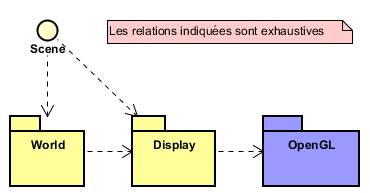
\includegraphics[scale=.6]{overview_uml}
	\caption{Diagramme de classes : composantes principales du projet}
\end{figure}


Nous avons passé un certain temps en amont sur la conception globale de l'application. Elle ressemble à ce qu'on trouverait dans un \textit{Game Engine} moderne du type Unity ou Unreal Engine. Il existe une unique \textit{scène} - un monde - qui contient des objets qui sont affichés et mis à jour régulièrement.

La scène est construite une seule fois et le joueur y existe et peut s'y balader. La scène est globalement statique, les seuls objets qui se déplacent sont le joueur et le soleil, le reste est figé en place mais peut être animé d'autres manières.

\begin{figure}[ht]
	\centering
	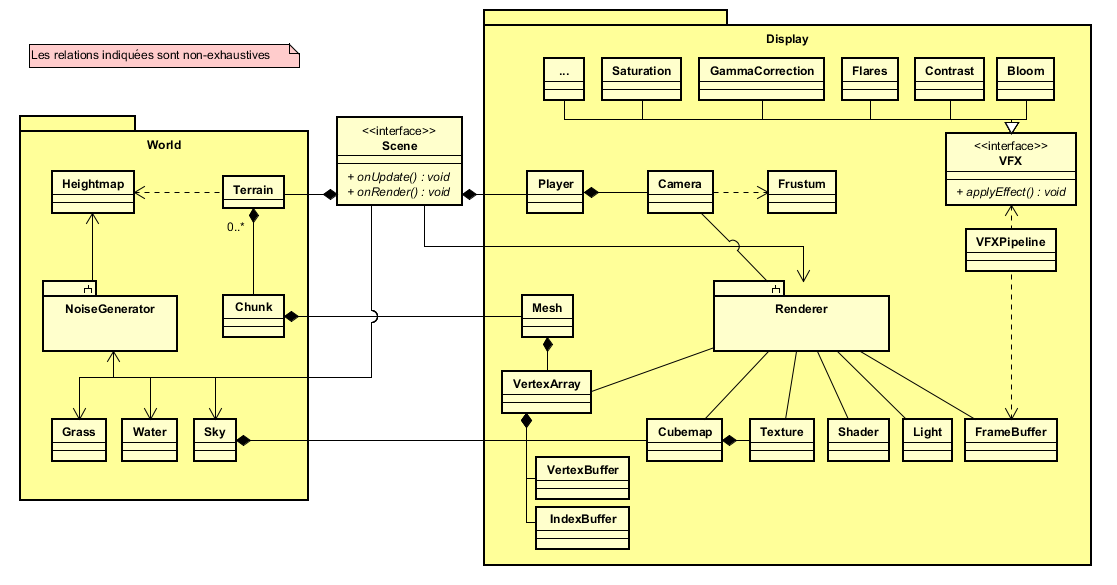
\includegraphics[scale=.49]{detailed_structure_uml}
	\caption{Diagramme de classes : composantes détaillées}
\end{figure}

\section{Tests, sandbox}

Ce genre de projet est très peu propice aux tests, pour s'assurer du bon fonctionnement global de l'application nous nous baserons sur des tests d'intégration seulement. Pour chaque fonctionnalité nous créerons une scène qui présentera seulement la fonctionnalité en question, de cette manière il sera très simple de vérifier le bon fonctionnement de chaque partie du système.

En plus de ces scènes de test, nous créerons des scènes \textit{sandbox} qui intégreront toutes les fonctionnalités et serviront de démonstrations techniques des résultats que nous obtiendrons. Voici la liste des scènes finales, dans l'ordre dans lequel nous les avons créé (il manque celles qui ont été retirées pendant le développement).

\paragraph{}
\begin{tabular}{|l|l|}
	\hline
	Nom de la scène & Fonctionnalité \\\hline\hline
	\code{TestCameras} & Caméra perspective, orthogonale, champ de vision\\\hline
	\code{TestShaders} & \hyperref[sec:shaders]{Vertex Shader et Fragment Shader}\\\hline
	\code{TestSky} & \hyperref[sec:sky]{Cubemap}, nuages\\\hline
	\code{TestTerrain} & \makecell[l]{Scène de tests principale, génération de terrain, érosion,\\ fonctions de bruit, brouillard}\\\hline
	\code{TestFB} & \hyperref[sec:framebuffers]{Frame buffer}, effets spéciaux\\\hline
	\code{TestComputeShader} & \hyperref[sec:shaders]{Compute shader}\\\hline
	\code{TestShadows} & \hyperref[sec:casted_shadows]{Ombres portées}, caméra orthogonale, depth map\\\hline
	\code{TestInstanced} & \hyperref[sec:instanced_rendering]{Instanced rendering}, affichage de l'herbe\\\hline
	\code{TestWater} & Réflexion, réfraction\\\hline
	\code{POC1} & Intégration - terrain, ombres\\\hline
	\code{POC2} & Intégration - terrain, herbe\\\hline
	\code{POC[3,4]} & Intégration - démonstrations de différents types de terrain\\\hline
\end{tabular}

\chapter{Génération de terrain}

Pour générer notre terrain, il nous faut d'abord lister les contraintes que nous nous fixons - et celles que nous ignorons - ; nous voulons :
\begin{itemize}
	\item{un grand terrain}
	\item{sans répétitions}
	\item{assez détaillé}
	\item{dont la hauteur change}
\end{itemize}

Nous nous restreindrons à une seule valeur de hauteur par position dans le plan, donc pas de grotte ou de surplomb. Les algorithmes classiques qui correspondent à ces critères consistent à créer une \textit{carte de hauteur} (\textit{heightmap}) et à placer des points sur une grille dont les hauteurs correspondent à celles de la carte. Il suffit ensuite de relier ces points pour avoir un terrain convaincant comme illustré par la figure \ref{fig:wireframe_terrain}. L'objet généré s'appelle un \textit{Mesh}.

\begin{figure}[ht]
	\centering
	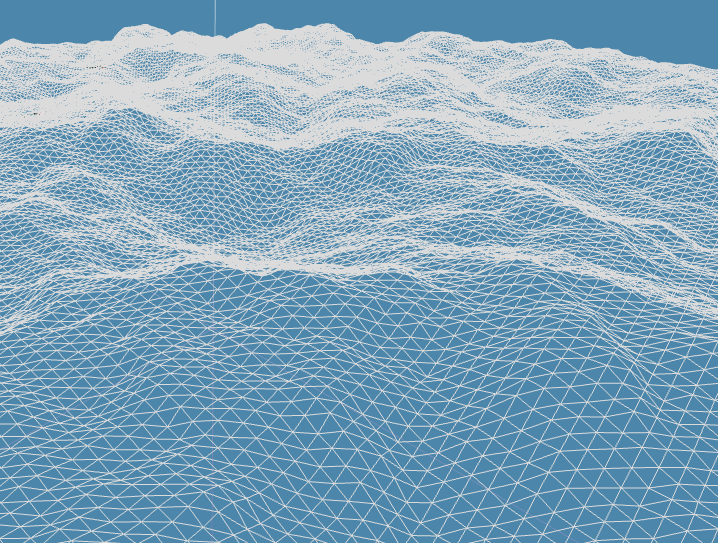
\includegraphics[scale=.49]{terrain_wireframe}
	\caption{Un mesh de terrain fait à partir d'une grille élevée}
	\label{fig:wireframe_terrain}
\end{figure}

Ici on a relié les points par des segments mais de manière générale on dessinera des triangles pleins.

Il existe d'autres méthodes pour faire ce genre de terrain (cubemarching, raymarching avec génération dynamique...) qui permettent de faire plus mais qui sont beaucoup plus gourmandes en performances et en complexité. Dans notre cas une heightmap est beaucoup plus adaptée.

\section{Bruit de Perlin}

Pour créer la heightmap il nous faut ce qu'on appelle un \textit{bruit}, une fonction dont le domaine de définition est le plan $xz$ et le domaine de valeurs est $\mathbb{R}$. Cette fonction doit être pseudo-aléatoire mais déterministe. La plus simple est le \textit{white noise} qui est "complètement aléatoire"\footnote{On utilisera le générateur de nombres pseudo-aléatoires de C++ pour attribuer une valeur à chaque point du plan $\mathbb{Z}^2$.}. On s'intéressera plutôt aux fonctions de bruit continues sur $\mathbb{R}^2$.

\begin{figure}[ht]
	\centering
	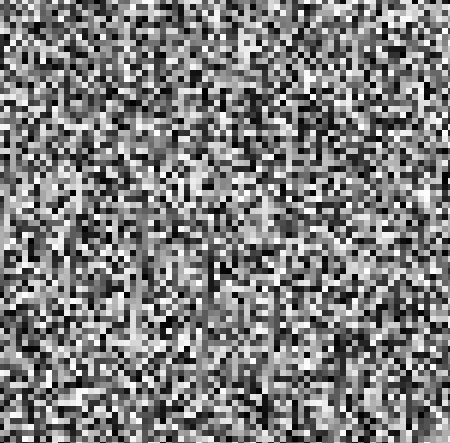
\includegraphics[scale=.49]{white_noise}
	
\includegraphics[scale=.49]{perlin_noise}
	\caption[White noise et Perlin noise]{White noise et Perlin noise\\Les pixels blancs sont plus hauts et les pixels\\ noirs sont plus bas une fois portés en 3D}
	\label{fig:noises}
\end{figure}

Les fonctions les plus communes pour une génération de ce style sont de la famille des \textit{Gradient noise} (bruit de gradient) et \textit{Value noise} (bruit de valeur).
Un value noise est défini à partir d'un white noise de cette manière :

\begin{alignat*}{3}
	V(x,y) =f( &f(B(\floor{x},\floor{y}), &&B(\floor{x+1},\floor{y}), &&\fract{x}),\\
			&f(B(\floor{x},\floor{y+1}), &&B(\floor{x+1},\floor{y+1}), &&\fract{x}),\\
			&\fract{y})
\end{alignat*}

Ici $V$ est le value noise, $B$ est le white noise et $fract(x)$ est la partie fractionnaire de $x$. $f$ dépend du value noise, c'est une fonction d'interpolation, la plus simple est l'interpolation linéaire\footnote{$lerp(a,b,x) = a+(b-a)\times x$}.
L'idée est d'interpoler entre des valeurs complétement aléatoires selon une grille. Le value noise permet de générer des heightmaps très simplement, mais qui laissent à désirer. Aujourd'hui il a été très largement remplacé par le bruit de Perlin, qui est un cas spécifique de gradient noise.

La différence avec le value noise est qu'au lieu d'utiliser un white noise comme base, on génère à la place une grille de vecteurs unitaires et pour calculer les "$B(x,y)$" on calcule le produit scalaire du point $(x,y)$ à l'intérieur de sa cellule sur la grille avec les vecteurs unitaires :

\begin{align*}
	fx&=\floor{x} & a_{00}&=<(dx,dy), U_{fx,fy}>\\
	fy&=\floor{y} & a_{10}&=<(dx-1,dy), U_{fx+1,fy}>\\
	dx&=\fract{x} & a_{01}&=<(dx,1-dy), U_{fx,fy+1}>\\
	dy&=\fract{y} & a_{11}&=<(1-dx,1-dy), U_{fx+1,fy+1}>
\end{align*}
\begin{alignat*}{3}
	G(x,y) =f( &f(a_{00}, &&a_{01}, &&dx),\\
			&f(a_{10}, &&a_{11}, &&dx), dy)
\end{alignat*}

Dans son article\cite{perlinnoise}, Ken Perlin défini le \textit{Simple gradient noise} avec $f$ l'interpolation linéaire, et le bruit de perlin, avec $f$ la fonction $smoothstep$\footnote{$smoothstep(a,b,x) = 3x^2-2x^3$}.

Ces bruits sont bons pour un terrain simpliste, mais l'astuce de Ken Perlin est d'en cumuler plusieurs octaves. En jouant sur la fréquence et l'amplitude de chacune :
\begin{align*}
	Height(x,y) = \sum_{k=1}^{N}&Amplitude_k G(Frequency_k\times(x,y))\\
	Amplitude_k &= Persistence^k\\ 
	Frequency_k &= Lacunarity^k
\end{align*}
Les paramètres qui nous restent à contrôler sont la persistance (le facteur de taille entre deux octaves), la lacunarité (le facteur de poids entre deux octaves) et le nombre d'octaves. Avec ceci on arrive à des cartes de hauteur assez réalistes, comme illustré en figure \ref{fig:layered_noise}. À noter que dans certains cas on préférera définir les amplitudes et fréquences par octave sans utiliser de persistance ou lacunarité.

\begin{figure}[ht]
	\centering
	
\includegraphics[scale=.3]{perlin_1_octave}
	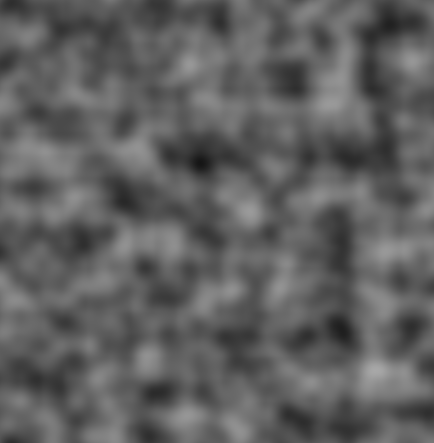
\includegraphics[scale=.3]{perlin_2_octaves}
	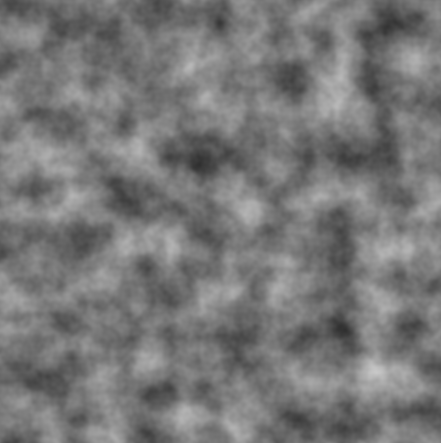
\includegraphics[scale=.3]{perlin_4_octaves}
	\caption{1, 2 et 4 octaves du Perlin noise}
	\label{fig:layered_noise}
\end{figure}

\subsection{Nuages}
Dans ce projet la première utilisation des fonctions de bruit est la génération du terrain, mais leurs utilités ne s'arrêtent pas ici. Une autre application évidente est la génération de nuages, on peut agrandir une de ces images, la placer au dessus du joueur et utiliser le niveau de blanc comme un niveau de transparence pour avoir des nuages très facilement. On peut même faire se déplacer les nuages en ajoutant un facteur $+Displacement_{k}$ à chaque octave avant d'appliquer $G$, en utilisant des facteurs plus importants pour les hautes octaves on obtient vite une animation de vent convaincante.

\section{Erosion}

On peut rendre le bruit généré plus réaliste encore en appliquant des propriétés physiques naturelles, la première à laquelle on pense est l'érosion.

L'idée est de simuler un très grand nombre de gouttes d'eau qui dévalent les pentes en arrachant des sédiments du terrain et en les relâchant en aval. L'algorithme que nous utiliserons est expliqué dans la thèse de Hans Theobald Beyer\cite{erosion}.
Dans le code cela consiste à calculer une suite de valeurs de gradient de la heightmap pour déplacer les gouttes selon la pente, et à chaque déplacement on calcule la quantité de sédiments à arracher ou déposer. Le seul bémol est que le dépot et l'érosion ne se font pas seulement à la position de la goutte, mais aussi aux alentours. Pour ne pas recalculer les différences à chaque étape de chaque goutte on fait le calcul en amont, qu'on stocke pendant toute la durée de l'algorithme. Cela peut poser certains problèmes de performance et de besoin en mémoire, l'espace mémoire nécessaire est en $O(n^2)$ avec la taille du terrain et le premier facteur du polynôme est très important.

\begin{figure}[ht]
	\centering
	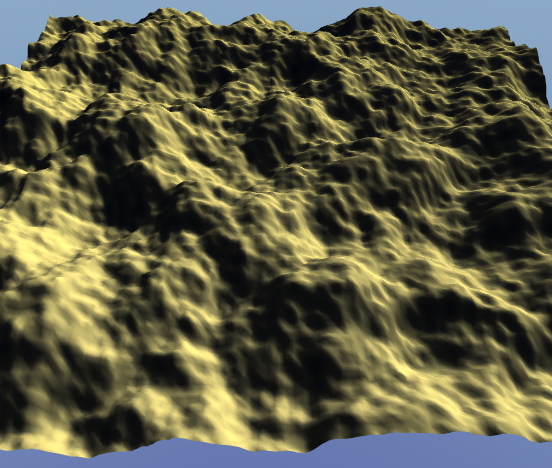
\includegraphics[scale=.4]{erosion_before}
	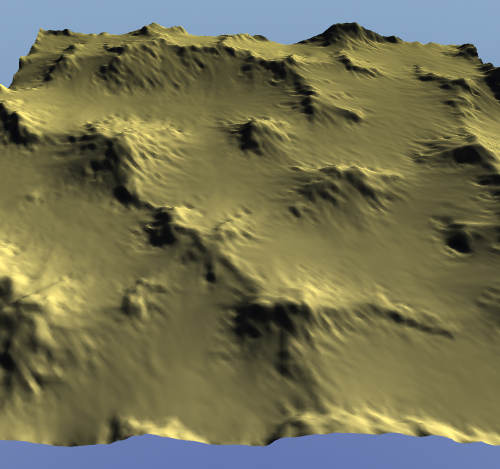
\includegraphics[scale=.4]{erosion_after}
	\caption{Comparaison avant/après application de l'érosion}
	\label{fig:erosion_comparison}
\end{figure}

\section{Structure du terrain}

On verra ensuite que penser à l'affichage du terrain avant de fixer sa structure est essentiel, avec une bonne structure l'affichage est plus simple et beaucoup plus performant. L'idée est que les données du terrain ne peuvent pas (ou peu) être modifiées pendant l'exécution mais qu'elle doivent pouvoir être segmentées pour n'en afficher qu'une partie.
Pour résoudre ce problème nous divisons le terrain en parcelles (\textit{chunks}). Chaque parcelle peut être générée et affichée indépendamment des autres, seul sa position suffit à savoir ce qu'elle contient.
Avec cette division il est assez simple de faire un terrain qui se met à jour en fonction de la position du joueur, pour que les chunks proches soient toujours visible.

%% classes



\section{Variations}

Avant de générer le mesh du terrain on peut modifier la heightmap pour obtenir différents résultats, on peut même ne pas utiliser les fonctions de bruit et la générer complètement différemment.

\begin{itemize}
	\item{À partir d'un bruit de Perlin de paramètres $N=2$ $Amplitude=[1, .5]$ $Frequency=[.3, .15]$ et en appliquant $h\rightarrow H-\abs{2x-H}$ on obtient un terrain qui ressemble aux dunes d'un desert.}
	\item{Dans une de nos scènes de démonstration nous appliquons $(x,y)\rightarrow Perlin(x,y)+\frac{S}{8}(\abs{x-\frac{S}{2}}+\abs{y-\frac{S}{2}})$ pour abaisser le terrain au centre sans que ce soit trop visible, simplement pour qu'à un bout de la carte on puisse voir davantage.}
	\item{On peut récupérer des cartes de hauteur de zones géographiques existantes (on en trouve sur internet\footnote{\url{https://tangrams.github.io/heightmapper}}).}
	\item{Avec un peu plus d'effort on peut créer des plateaux et arriver à une génération ressemblant aux Mesa}
\end{itemize}

Des illustrations de ces variations peuvent être trouvées en \ref{fig:final}.


\chapter{Affichage 3D}

L'affichage représente la plus grosse partie du projet, on a beau avoir un terrain immense et avec des détails très fins, s'il est impossible de l'afficher le tout n'a plus grand intérêt.

Nos contraintes principales seront de pouvoir afficher un très grand terrain, avec des performances qui permettent le déplacement en temps réel (60 images par secondes). Concrètement cela veut dire qu'afficher une image doit prendre moins de 16.6ms, ce qui peut être très difficile à respecter dans certains cas.

Avec ces considérations et notre expérience passée commune, nous avons choisi d'utiliser OpenGL comme interface avec le gpu (carte graphique).

\section{OpenGL}

OpenGL est une spécification qui définit des points d'entrée d'une interface cpu-gpu. Pour utiliser OpenGL nous avons besoin d'une librairie dépendante du langage de programmation ; en c++ nous utiliserons glad. Nous aurons aussi besoin de librairies pour la gestion de la fenêtre de l'application et l'interface utilisateur, nous utiliserons glfw et ImGui.


\paragraph{}
OpenGL fonctionne comme une \textit{state machine}. Chaque fonction modifie l'état interne du gpu et certaines lances des commandes à exécuter comme l'affichage de formes géométriques.
Il est important de mentionner que les gpu modernes ne savent pas afficher autre chose que des triangles et des lignes, pour afficher un rectangle on devra se contenter de dessiner deux triangles.

\section{Shaders}
\label{sec:shaders}

Les \textit{shaders} sont des programmes qui tournent sur le gpu plutôt que sur le cpu. Nous utiliserons extensivement deux types de shaders pour l'affichage : le \textit{vertex shader} qui s'exécute pour chaque sommet des triangles affichés ; et le \textit{fragment shader} qui s'exécute pour chaque pixel couvert par le triangle. Des shaders classiques ressemblent au code en \ref{fig:vs_fs_shaders}.


\begin{figure}[ht]
	\centering
	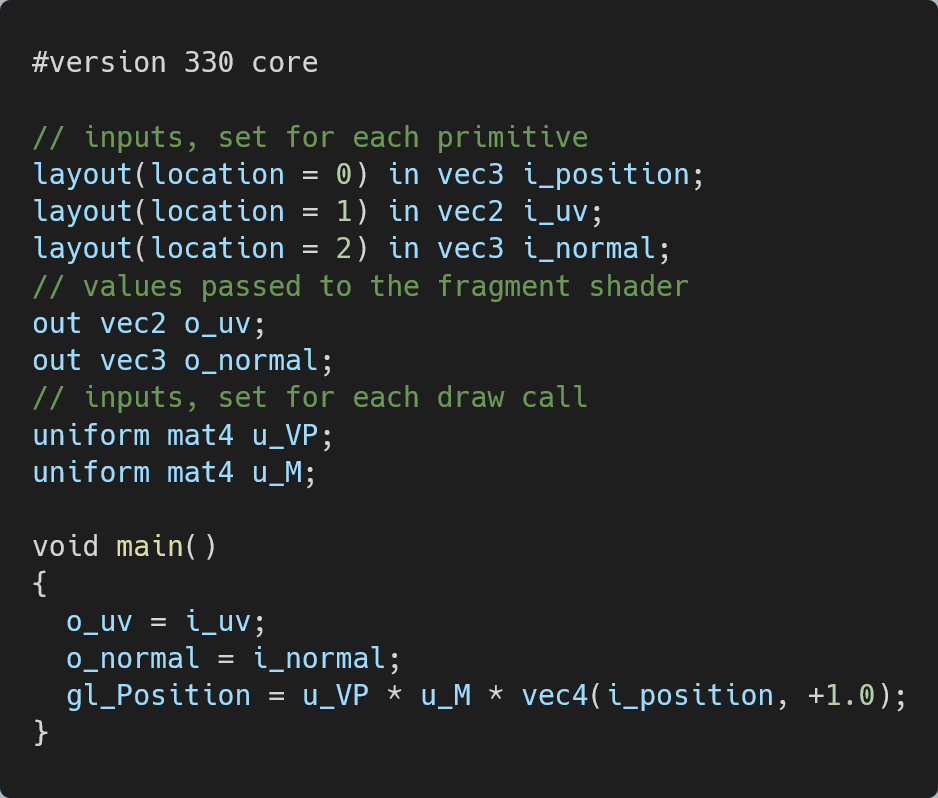
\includegraphics[scale=.2]{vertex_sample}
	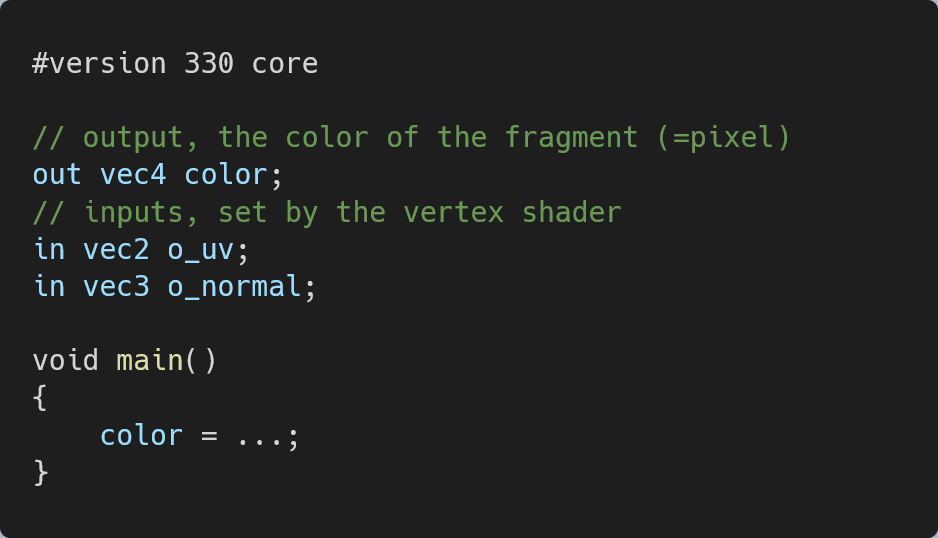
\includegraphics[scale=.2]{fragment_sample}
	\caption{Exemple de Vertex Shader et Fragment Shader}
	\label{fig:vs_fs_shaders}
\end{figure}

Un dernier type de shader que nous utiliserons est le \textit{compute shader}, qui ne sert pas à l'affichage mais permet de faire des calculs massivement parallèles sur le gpu. Il nous sera utile pour gagner en performance.
\par
Chaque shader prend des entrées différentes, ce qui est commun à tous c'est la notion d'\textit{uniform} : des variables globales qui peuvent être changées seulement entre deux appels à des fonctions d'affichage/d'exécution de compute shader.
Avec ces éléments définis on peut faire un schéma de la "pipeline OpenGL"  comme illustré en figure \ref{fig:opengl_pipeline}.

\begin{figure}[th]
	\centering
	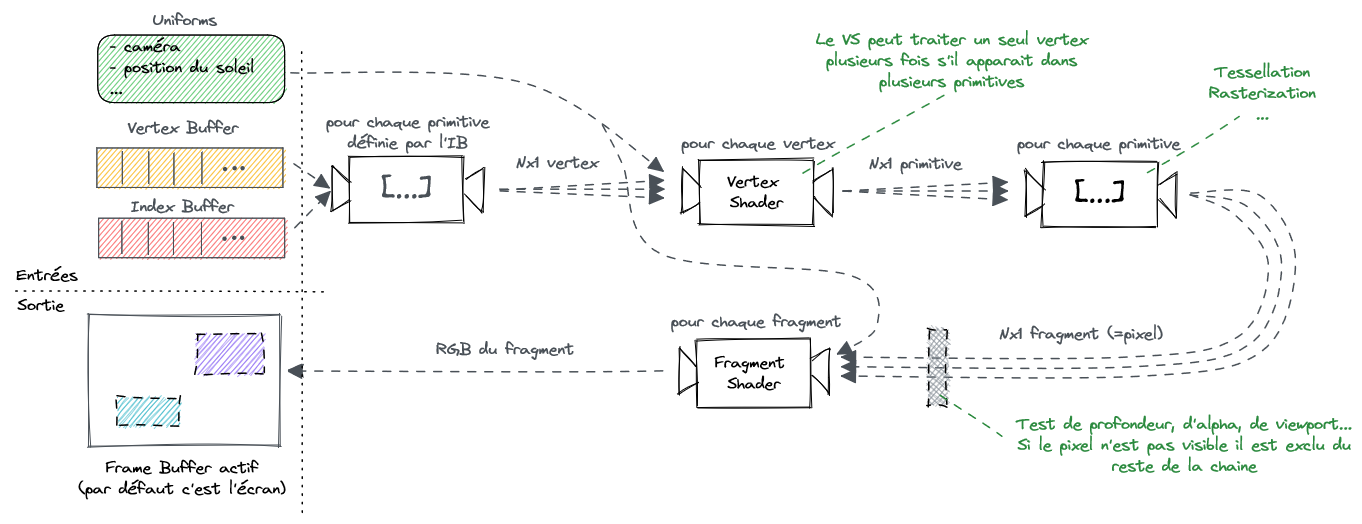
\includegraphics[scale=.3]{opengl_pipeline}
	\caption{Schéma de la pipeline OpenGL}
	\label{fig:opengl_pipeline}
\end{figure}

\section{Repères, caméras et mathématiques}

Avant de pouvoir afficher quoi que ce soit à l'écran, il nous faut des données à afficher (Vertex Buffer et Index Buffer, nous y reviendrons \hyperref[sec:instanced_rendering]{plus tard}), des shaders pour définir \textit{comment} l'afficher et aussi bien comprendre comment placer les triangles à l'écran.
Par défaut OpenGL utilise un \textit{viewport} (un espace virtuel d'affichage) compris entre $-1$ et $1$ en $x$ et $y$ et entre $0$ et $1$ pour $z$. Cela signifie que la position générée par le Vertex Shader doit être comprise dans cet intervalle pour que le pixel associé être affiché (le vertex shader définit la position des sommets, les positions des pixels du triangle en sont déduites). Un sommet de coordonnées $(-1,-1,0)$ est affiché en haut à gauche de l'écran et un sommet $(1,1,0)$ est affiché en bas à droite. La coordonnée $z$ est utilisée pour la profondeur.
\par
Nous définirons deux repères supplémentaires, celui du monde (dans $\mathbb{R}^3$) et celui des modèles (dans $\mathbb{R}^3$). Imaginons qu'on veuille afficher le modèle d'un arbre, on va d'abord créer les sommets dans le repère du modèle (centré en $(0,0,0)$, aux dimensions 1:1), on le transformera pour passer dans le repère du monde (d'abord une mise à l'échelle puis une translation pour le placer au bon endroit) et enfin on le projetera sur le viewport, la projection dépendra du type de caméra qu'on utilisera.

Un gros avantage de cette méthode est que toutes ces transformations sont des opérations de projection d'un espace à un autre, qu'on peut donc les décrire avec des multiplications de matrices. En mémoire il nous suffira de conserver les positions dans le repère du modèle et les deux matrices de changement de repère.

\paragraph{}
Un exemple : on veut doubler la taille d'un modèle puis le déplacer de deux unités dans le sens $+x$, on applique la transformation suivante à chacun de ses points.
$$
	P = \begin{pmatrix}x\\y\\z\\1\end{pmatrix}\\
	A = \begin{pmatrix}2&0&0&0\\0&2&0&0\\0&0&2&0\\0&0&0&1\end{pmatrix}\\
	B = \begin{pmatrix}1&0&0&2\\0&1&0&0\\0&0&1&0\\0&0&0&1\end{pmatrix}\\
$$
$$
	BAP = \begin{pmatrix}2x+2\\2y\\2z\\1\end{pmatrix}
$$

\begin{wrapfigure}{R}{0.3\textwidth}
	\begin{center}
	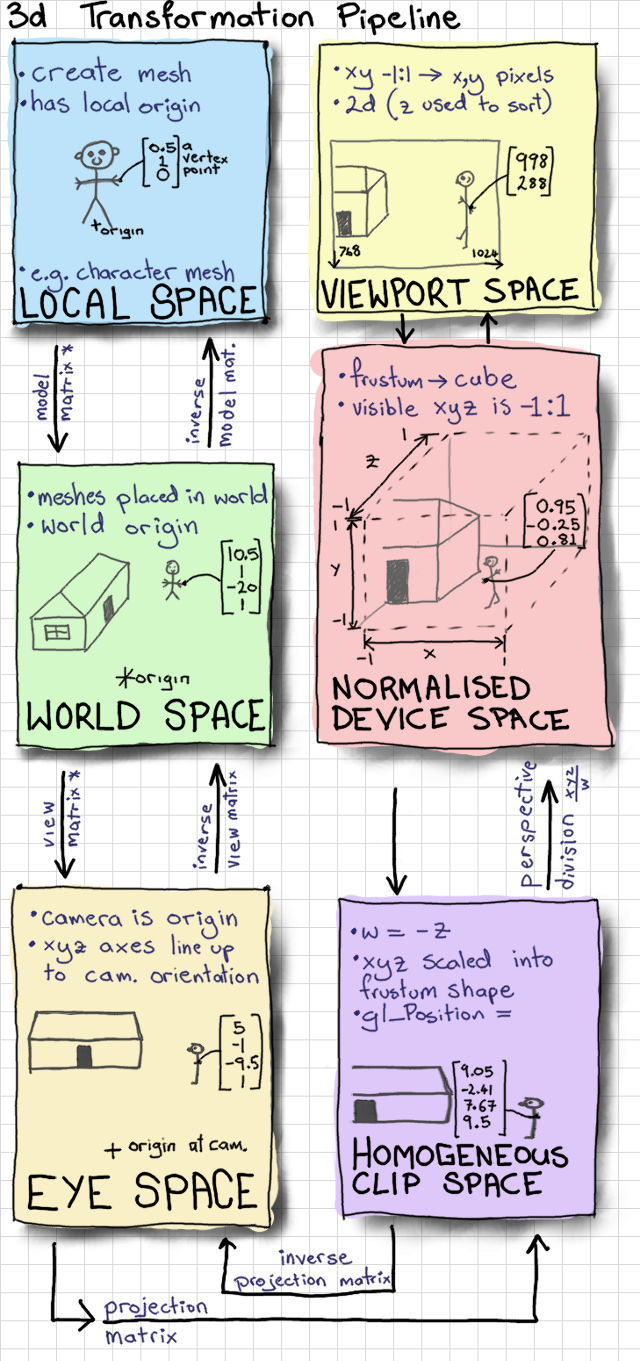
\includegraphics[scale=.2]{coordinate_systems}
	\end{center}
	\caption[Résumé des repères]{Résumé des repères\\\url{https://www.aosabook.org/en/500L/a-3d-modeller.html}}
	\label{fig:coordinate_systems}
\end{wrapfigure}

Ici $A$ est une matrice de mise à l'échelle et $B$ est une matrice de translation, $C=BA$ serait la matrice de transformation (projection) du repère modèle au repère monde. La quatrième coordonnée est utilisée pour faciliter le calcul des translations, elle vaudra toujours $1$ pour les points et $0$ pour les vecteurs même s'il est plus rare de faire ces projections sur des vecteurs.


\paragraph{}
La projection du monde vers le viewport est un peu plus compliquée, il existe deux types principaux de projection qui sont les projections perspective et orthogonale. Elles possèdent chacune une écriture matricielle que nous ne détaillerons pas mais qui peuvent se retrouver assez facilement avec un peu d'algèbre linéaire. Cette projection seule ne suffit pas, tel quel notre caméra devrait toujours être placée à l'origine du monde et être dirigée selon l'axe $+x$...
\par


\paragraph{}
Une astuce pour prendre en compte la position de la caméra est d'appliquer une transformation au repère du monde qui projète la caméra à l'origine et dirigée vers $+x$, de cette manière nous n'avons pas à modifier la dernière projection. Par exemple si la caméra est située en $(2,3,4)$ on appliquera $(x,y,z)\rightarrow(x-2,y-3,z-4)$ à tous les points avant de les projeter sur le viewport (ici on ne tient bien sûr pas compte de la rotation de la caméra).

\paragraph{}
Pour finir on retient trois matrices de projection :
\begin{itemize}
	\item{$M$ ("model") qui transforme du modèle au monde}
	\item{$V$ ("view") qui annule la transformation de la caméra}
	\item{$P$ ("projection") qui projète du monde au viewport}
\end{itemize}

Ce modèle en trois matrices est le plus utilisé. Il suffit de donner $P'=PVM$ au Vertex Shader et lui laisser transformer chaque vertex. On notera d'ailleurs qu'il suffit d'inverser $P'$ pour projeter des positions à l'écran à des positions dans le monde, on peut par exemple savoir où - dans le monde - l'utilisateur pointe lorsqu'il clique à l'écran\footnote{Le calcul est un peu plus compliqué, on passe de $\mathbb{R}^2$ à $\mathbb{R}^3$, il faut tirer un rayon depuis la position de la caméra en direction du point qu'on vient de calculer à partir de $P'^{-1}$ et trouver la première intersection avec un objet du monde.}.

\section{Ciel}
\label{sec:sky}

Pour afficher le ciel il existe un objet assez spécifique qui s'appelle \textit{cubemap}. L'idée est d'afficher autour du joueur une texture de ciel, on pourrait théoriquement le faire en affichant une sphère - c'est ce qui serait le plus naturel - mais puisque nous sommes restreints à dessiner des triangles cela impliquerait de dessiner un \textit{très} grand nombre de triangles. On utilise donc une cubemap, qui est une projection d'une texture sphérique sur un cube, on peut ensuite afficher un cube plutôt qu'une sphère autour du joueur. Le calcul de projection inverse est fait directement par OpenGL.

Une optimisation qu'on retrouve à plusieurs autres moments est d'afficher ce ciel \textit{après} avoir affiché tout le reste, cela ne semble pas naturel mais en affichant seulement là où rien d'autre n'a été affiché on est sûr de ne pas dessiner des pixels inutiles. Le résultat est apparent en figure \ref{fig:sky_depth_test}.

\begin{SCfigure}
	\centering
	\caption[Zone dessinée en ordonnant les affichages]{Zone dessinée en ordonnant les affichages\\La region dessinée (le ciel) ne couvre qu'une partie de l'écran, c'est autant de travail de moins pour le gpu}
	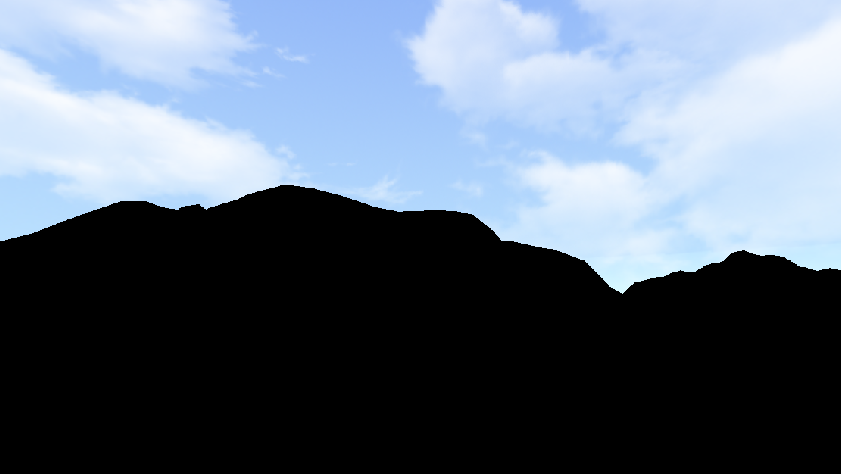
\includegraphics[scale=.45]{sky_depth_test}
	\label{fig:sky_depth_test}
\end{SCfigure}

\section{Ombres}

Nous avons implémenté deux types d'ombre : les ombres ambiantes et les ombres portées. Les deux se combinent très facilement dans le fragment shader utilisé pour le terrain.
\subsection{Ombre ambiantes}
Une ombre ambiante est l'obsurcissement des surfaces qui ne sont pas dirigées vers le soleil. Mathématiquement cela se calcule très bien à partir des normales du terrain, pour chaque pixel on calcule ce que reçoit le pixel :
$$ S_{ambiant}=max(0, \vec{N}\cdot \vec{D}) $$
Avec $\vec{N}$ la normale du terrain à la position du pixel, $\vec{D}$ la direction des rayons su soleil comme illustré dans la figure \ref{fig:ambiant_shadows_schema}.

\begin{figure}[ht]
	\centering
	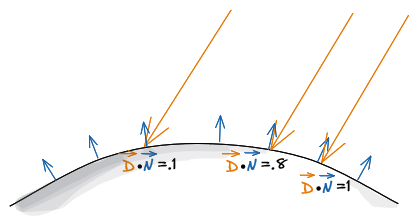
\includegraphics[scale=.49]{ombres_ambiantes}
	\caption{Schéma du fonctionnement des ombres ambiantes}
	\label{fig:ambiant_shadows_schema}
\end{figure}

\subsection{Ombre portées}
\label{sec:casted_shadows}
Le calcul des ombres portées est autrement plus compliqué, et se divise en plusieurs étapes
\begin{enumerate}
\itemsep-.5em
\item positionner le soleil pour qu'il éclaire le moins possible
\item afficher la scène "depuis le point de vue du soleil"
\item afficher la scène normalement, en tenant compte de la distance des objets au soleil
\end{enumerate}

\begin{figure}[ht]
	\centering
	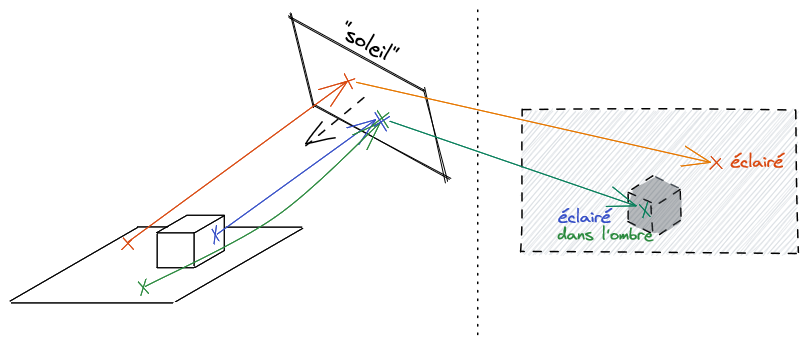
\includegraphics[scale=.49]{ombres}
	\caption{Schéma du fonctionnement des ombres portées}
	\label{fig:shadows_schema}
\end{figure}

L'idée est de calculer la distance des pixels au soleil et de vérifier que cette distance est bien la plus petite à la position du pixel du point de vue du soleil (en bleu et orange sur la figure \ref{fig:shadows_schema}), si ce n'est pas le cas cela signifie qu'un autre objet est plus proche du soleil et donc qu'il projète une ombre sur le pixel (en vert sur le schéma).

\paragraph{}
Le positionnement se fait en listant les objets qui doivent recevoir et pouvoir projeter des ombres. Tous les éléments qui ne sont pas dans le champ de vue du joueur n'ont pas à être éclairés mais ceux qui peuvent projeter des ombres sur des objets visibles doivent être pris en compte.

\begin{SCfigure}
	\centering
	\caption[Capture du positionnement de la caméra "soleil"]{Capture du positionnement de la caméra "soleil"\\Le trait rouge est la direction des rayons du soleil ; le plus grand pavé jaune est la zone visible par le joueur ; le pavé gris est la zone couverte par le champ de vision du soleil et les autres pavés sont en jaune s'ils n'influencent pas la position du soleil ou en rouge s'ils sont susceptibles de projeter une ombre sur la zone visible.}
	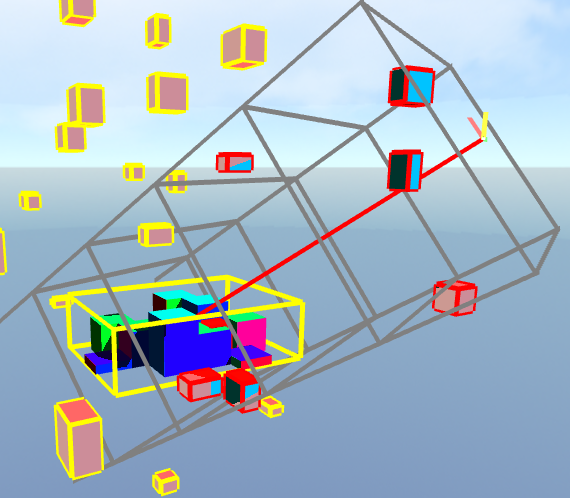
\includegraphics[scale=.49]{casted_shadows}
	\label{fig:sun_camera_position}
	\vspace{-10pt}
\end{SCfigure}

\paragraph{}
L'affichage de la scène depuis le point de vue du soleil utilise une caméra orthogonale car tous les rayons sont perpendiculaires. La distance la plus faible est enregistrée pour chaque pixel et est utilisée ensuite. La distance enregistrée ainsi est normalisée (linéarisée dans $[0,1]$) par OpenGL. La texture qui contient ces distances est appellée \textit{depth map} (\textit{carte de profondeur}).

\begin{SCfigure}
	\centering
	\caption[Depth map]{Depth map\\Les zones blanches sont loin de la caméra, les zones foncées sont plus proche. Les valeurs réelles de distance dépendent de la configuration de la caméra.}
	\fbox{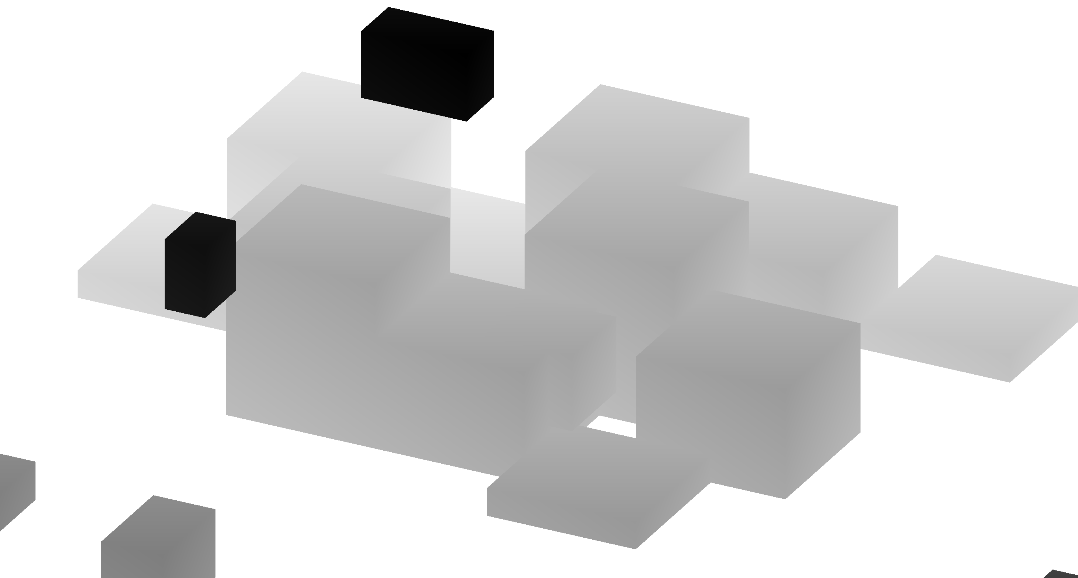
\includegraphics[scale=.25]{depth_map}}
	\label{fig:sun_depth_map}
	\vspace{-10pt}
\end{SCfigure}

Le calcul du positionnement de la caméra du soleil est la partie la plus compliquée de cet algorithme, nous ne le détaillerons pas ici mais le code peut être trouvé dans le fichier \code{SunCameraHelper.cpp}. Il s'agit surtout de projections de calcul de \textit{bounding boxes} et \textit{bounding spheres}.

\subsection{Algorithme final}

Après que la depth map ait été calculée, on arrive à l'algorithme \ref{alg:shadows} pour calculer la quantité de soleil que reçoit chaque pixel.
\begin{algorithm}
\caption{Calcul des ombres par pixel}
\label{alg:shadows}
\begin{algorithmic}
\State $P_s \gets \text{... matrice de projection monde$\rightarrow$depth map}$
\State $DM \gets \text{... depth map 2D}$
\State $\vec{D} \gets \text{... direction des rayons du soleil}$
\\
\State $\vec{p} \gets \text{...  position 3D du pixel}$
\State $\vec{n} \gets \text{... normale 3D à la position du pixel}$
\\
\State $S_{ambiant} \gets max(0, \vec{n}\cdot \vec{D})$
\State $\vec{u} \gets P_s\times\vec{p}$
\State $d_{pixel} \gets \vec{u}.z$
\State $d_{nearest} \gets DM(\vec{u}.xy)\times(z_{far}-z_{near})+z_{near}$
\State $S_{casted} \gets smoothstep(-\epsilon, 0, d_{pixel}-d_{nearest})$
\State $Q \gets S_{ambiant}\times S_{casted}$
\\
\State $PixelColor\gets mix(SunDarkColor, SunLightColor, max(.1, Q\times SunStrength))$
\end{algorithmic}
\end{algorithm}

On préfère utiliser la fonction $smoothstep$ et utiliser $\epsilon$ plutôt que de mettre $S_{casted}$ à $0$ ou $1$ pour éviter le crénelage du aux erreurs d'arrondis. Le résultat de ces algorithmes peut être vu en figure \ref{fig:shadows}.

\begin{SCfigure}
	\centering
	\caption[Capture des ombres]{Capture des ombres\\Il reste quelques soucis de crénelage, il existe des solutions (\textit{multisampling}) mais puisque notre cas d'utilisation est d'afficher la silhouete du terrain le crénelage n'est pas très génant.}
	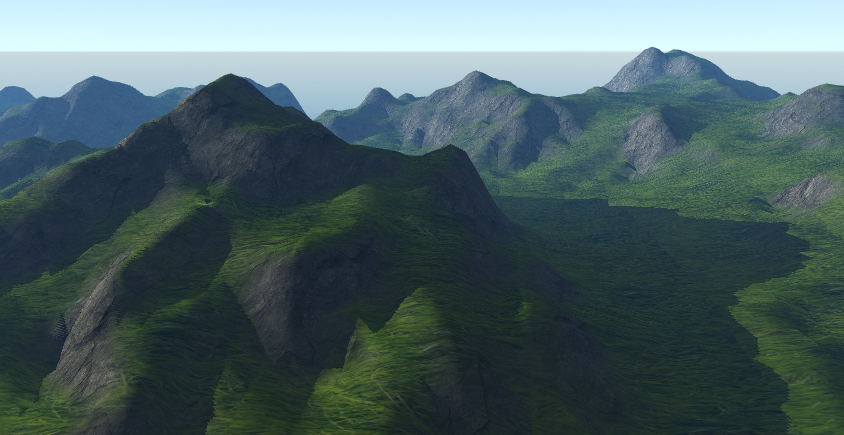
\includegraphics[scale=.45]{shadows}
	\label{fig:shadows}
	\vspace{-10pt}
\end{SCfigure}

\section{Instanced rendering}
\label{sec:instanced_rendering}

En plus du terrain en lui-même, nous avons choisi d'afficher quelques objets. Et par "quelques" il faut entendre plusieurs millions. Nous nous sommes donné le but d'afficher des brins d'herbe, nous reviendrons sur les algorithmes d'optimisation mis en place mais avant de pouvoir en discuter il est important de comprendre \textit{comment} OpenGL gère l'affichage.
\paragraph{}
Pour afficher un objet simple (un cube par exemple) il nous faut 4 structures de données sur le gpu : un \textit{Vertex Buffer}, qui contient les données de chaque sommet du cube ; un \textit{Index Buffer}, qui définit les triangles à partir des sommets ; un shader et un \textit{Vertex Array} que nous passerons sous silence car il n'influence pas les données.

Une manière très naïve d'afficher un très grand nombre d'éléments est de construire un Vertex Buffer (VB) et un Index Buffer (IB) par objet. Le souci est qu'à l'affichage il nous faudra changer le contexte OpenGL (modifier les VB/IB actifs) pour chaque élément, ce qui ralentit considérablement le tout\footnote{Le vrai problème vient du nombre d'appels à des fonctions d'affichage, il est possible d'afficher beaucoups d'éléments d'un coup mais seulement si le contexte n'a pas à changer}.
Si les objets sont identiques on peut n'utiliser qu'un seul IB, mais ce n'est pas suffisant.

\paragraph{}
Une manière déjà plus intéressante est de construire un unique VB qui contient tous les sommets de tous les éléments et un IB qui contient les triangles constitués de ces sommets, cela améliore déjà considérablement les performances. Cette méthode est appelée \textit{batch rendering}.
Cette méthode possède cependant un désavantage majeur, il est quasiment impossible de n'afficher qu'une partie des éléments. Pour le terrain par exemple nous n'affichons que les chunks visibles par la caméra, le batch rendering n'est donc pas adapté. On préférera faire des chunks de grande taille pour diminuer le nombre de changement de contextes même si cela diminue l'efficacité de n'afficher que les chunks visibles.

\paragraph{}
Dans notre cas on peut encore faire mieux, tout nos éléments sont identiques mis à part leurs positions dans le monde, on peut donc utiliser un seul VB et IB qui contiennent les données d'un unique brin d'herbe et le dessiner autant de fois que nécessaire à des positions différentes. Mais pour ne pas avoir à modifier le contexte OpenGL il faut que ces données d'instances soient présentes sur le gpu. On créé donc un \textit{instance buffer} qui contient la position de chaque brin d'herbe. Cette méthode s'appelle l'\textit{instanced rendering}.

\begin{figure}[ht]
	\centering
	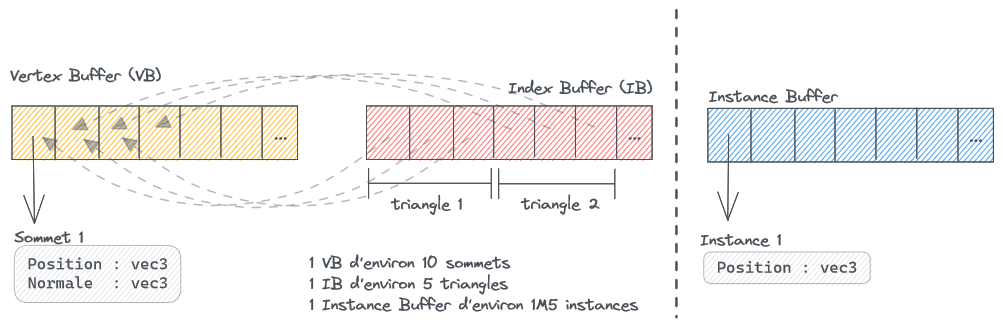
\includegraphics[scale=.4]{grass_vbibib}
	\caption{Structures présentes sur le gpu en instanced rendering}
	\label{fig:grass_vbibib}
\end{figure}

\subsection{Profilage}
Avec l'instanced rendering on peut afficher plusieurs centaines de milliers de triangles sans trop impacter les performances, mais ce n'est pas suffisant pour les quelques millions que nous nous sommes fixé, nous reviendrons sur les deux optimisations majeures dans la section \ref{section:grass_rendering}.
\paragraph{}
 Pour vérifier que notre implémentation est déjà meilleure que la naïve on peut comparer le temps mit avec les deux méthodes. Le profilage doit se faire avec des outils adaptés et non pas depuis C++ car le gpu et le cpu ont des fils d'exécution très différent\footnote{Nous utiliserons RenderDoc (\url{https://renderdoc.org/}) car il offre le plus d'outils compatibles avec OpenGL.}.

\begin{wrapfigure}{R}{0.3\textwidth}
	\begin{center}
		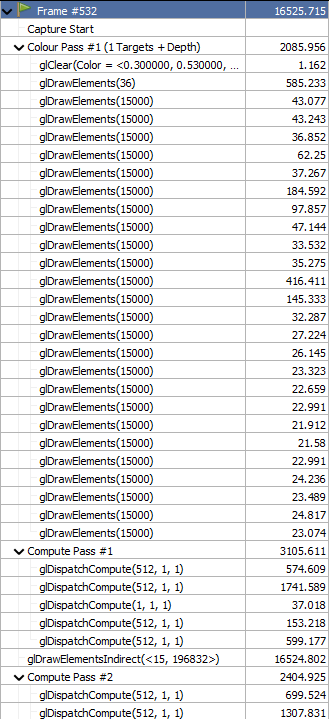
\includegraphics[scale=.4]{profiling}
	\end{center}
	\caption{Session de profiling avec RenderDoc}
	\label{fig:profiling}
\end{wrapfigure}

Le profilage répertorie l'ensemble des appels aux fonctions d'affichage (\code{glDrawXX}), les appels aux compute shaders (\code{glDispatchCompute}) et tous les appels de changement d'état (\code{glBindBuffer}, \code{glBindTexture}, \code{glUniformXX}... ces appels ont été masqués sur la figure \ref{fig:profiling} car leurs temps d'exécution sont négligeables). Le temps d'exécution pour chaque fonction indiqué en $\mu$s et le temps total ne doit pas dépasser $10^6/60=16666.\overline{6}\mu\text{s}\cdot$.



\section{Effets spéciaux}

\subsection{Frame Buffers} %% ...
\subsubsection{Frame Buffers} %% ...

\label{sec:framebuffers}


\paragraph{}
Un Framebuffer est un objet assez particulier mais incontournable des librairies graphiques, dont OpenGL.
La manière la plus simple de se représenter un framebuffer, c'est de se dire qu'on va rediriger OpenGL pour qu'il fasse tous ses dessins dans une texture cible, celle qui est attachée à notre framebuffer. On peut ensuite récuperer cette texture et s'en servir comme une nouvelle image.

Il y a par défaut deux Framebuffers : celui dans lequel OpenGL dessine, puis celui qui est affiché. On doit, à chaque itération de notre boucle principale, appeler explicitement la fonction glSwapBuffers() qui dit à OpenGL d'inverser ces textures.
En soit, l'image qu'on voit sur l'écran est toujours une frame en retard ; celle sur laquelle on travaille est "cachée".

On peut donc définir nous même des framebuffers qui permettent, bien souvent, de prendre notre scène en "photo" pour y appliquer un tas de modifications, à la manière des logiciels de retouche.
Cependant, on ne peut plus avoir accès à la géometrie de ce qui est écrit dans le framebuffer, donc on peut avoir des problèmes de profondeur.
Pour palier à ca, on peut utiliser un Z-buffer ou Depth-Buffer. Il s'agit d'un framebuffer dans lequel on inscrit la distance entre un pixel et la caméra. Nous l'avons vu plus haut dans la section \ref{sec:casted_shadows} concernant les ombres projetées.


%% IMAGE Z BUFFER?

\subsubsection{Pipeline VFX} %% ...

A l'aide de ces framebuffers, on peut donc appliquer des retouches après le calcul de la géométrie : on parle alors de Post-Processing.
Ces effets de post-processing font partie de la catégorie des effets spéciaux (Visual Effects - VFX). 

Il faut également savoir que l'application des différents effets spéciaux diffère selon l'ordre. On peut facilement s'en convaincre avec des inversions et multiplications de couleurs sur les pixels.
Ainsi, on définit une Pipeline d'effets : une pipeline prend une entrée, applique tout un tas d'opérations, et nous ressort l'entrée modifiée.

Dans notre cas, on définie une classe abstraite VFX qui implémente forcément une méthode qui prend une texture en entrée et lui applique l'effet que la classe fille représente.
La pipeline contient alors un ensemble de VFX - que l'utilisateur choisit ou non d'ajouter à sa scène - et qui, chacun leur tour, vont appliquer leur effet. pour finalement dessiner la texture modifiée à l'écran.

Voici une liste d'effets spéciaux que nous avons implémenté.

\paragraph{}

\begin{table}[H]
\centering
\begin{tabular}{|l|l|}
	\hline
	Nom de l'effet & \makecell{Résultat produit \\ }\\\hline\hline
	\code{Contrast} & \makecell{Accentuation des couleurs des pixels} \\\hline
	\code{Gamma Correction} &\makecell{ Balance des fortes valeurs de blanc} \\\hline
	\code{Saturation} & \makecell{Accentuation des fortes couleurs de pixels} \\\hline
	\code{Sharpness} & \makecell{Effet d'amélioration de netteté\\ et de démarquation des bordures}\\\hline
	\code{Sun Flares} & \makecell{Mimique de l'effet de surexposition\\ qui donne des halos lumineux\\lorsqu'une caméra regarde le soleil}\\\hline
	\code{Lens Mask} & \makecell{Mimique des fines poussières sur le verre\\ des vraies caméras}\\\hline
	\code{Bloom} & \makecell{Effet de saignement de la lumière qui provient\\ sur des sources très lumineuses}\\\hline
\end{tabular}

\end{table}

%% TODO IMAGE RECAPITULATIVE

\subsubsection{Bloom} %% ...


\paragraph{}
Parler du bloom permet de comprendre un concept clé des effets spéciaux : l'HDR.\\
HDR veut dire High Dynamic Range, en opposition au Low Dynamic Range (LDR).\\\\
On explique souvent cela comme : "Les valeurs R,G,B des pixels peuvent aller au dela de 1". C'est exactement ca, mais c'est difficile de comprendre à quoi ca sert ! \\\\
Le HDR s'active en donnant plus de bits par pixels : au lieu d'avoir 24bits, ou 8 bits par channel (soit les fameux 255 valeurs possibles par channel), on passe à 32 bits.\\
Très souvent, on donne 10 au rouge, et 12 au vert / bleu : c'est simplement que l'oeil humain percoit moins bien les nuances de rouge.

\paragraph{}
On sait qu'un pixel (1,1,1) est blanc en LDR.  Et c'est pareil en HDR ! Si on donne maintenant un pixel (2,2,2), il est aussi blanc !
Peut importe ce qu'on veut, quand les couleurs sont affichées à l'écran, elles ont forcément été restreinte entre 0 et 1.
Le HDR permet garder des informations et de donner plus de précision quand aux couleurs dominantes d'une lumière : l'exemple typique est celui du sabre laser.
Un sabre laser est blanc : il est tellement lumineux qu'il est blanc. Et pourtant, il a une aura autour de lui qui lui donne sa couleur ! Au fur et à mesure que la lumière diminue, les couleurs dominantes sont revelées.
Ainsi, un pixel (15,1,1) est blanc, mais en théorie, il devrait émettre dans le rouge.


\paragraph{}
C'est cet effet que le bloom reproduit. En filtrant les pixels les plus lumineux de l'écran, ceux qui sont fondamentalements blancs, mais dont les valeurs excèdent 1, on peut savoir quels sont les zones qui sont censé avoir un halo lumineux à cause de la dissipation de la lumière.
Pour implémenter cet effet, le standard dans l'industrie du jeu-vidéo provient de \textit{Call Of Duty : Modern Warfare}\cite{bloom}.\\
L'idée est de prendre la scène en photo, puis de diviser par 4 sa résolution tout en appliquant un calcul de ponderation des pixels, qui permettent de, peu à peu, faire ressortir les couleurs dominantes des zones lumineuses.
On effectue cette opération 5 ou 6 fois, et puis on se retrouve avec une image très petite (~15x20 pixels). On va maintenant faire l'inverse, et additioner peu à peu ces textures : l'addition d'une texture $i$ avec la texture $i-1$ permet de donner un effet de flou et d'attenuation.
Enfin, au terme de tout ca, après environ 13 calculs, on obtient une image avec des halos lumineux !

\begin{figure}[ht]
	\centering
	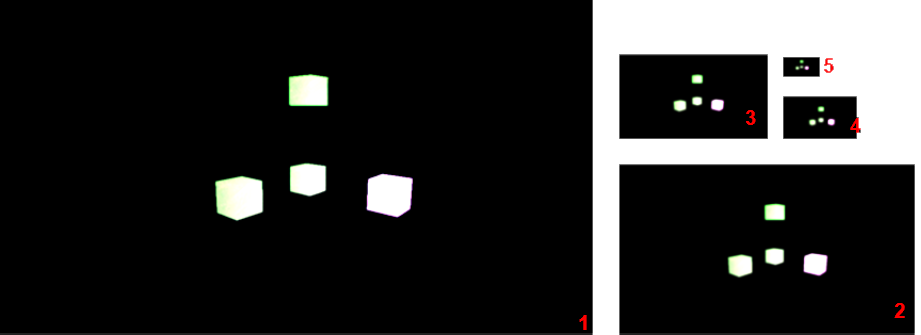
\includegraphics[scale=.5]{down_samples}
	\caption{Filtrage des pixels lumineux, et procédé de réduction de résolution des textures}
	\label{fig:bloom_down_sample}
\end{figure}

\begin{figure}[ht]
	\centering
	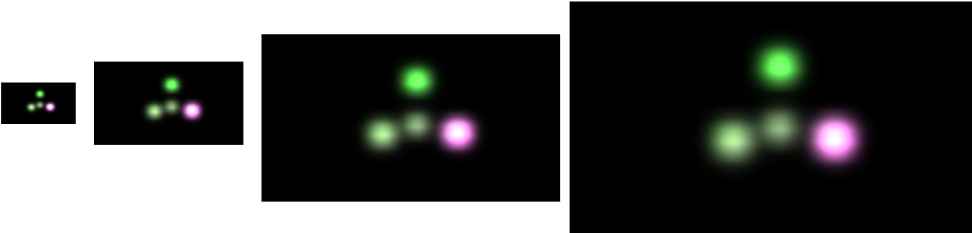
\includegraphics[scale=.7]{up_samples}
	\caption{Addition des textures pour obtenir un flou}
	\label{fig:bloom_up_sample}
\end{figure}


\begin{figure}[H]
	\centering
	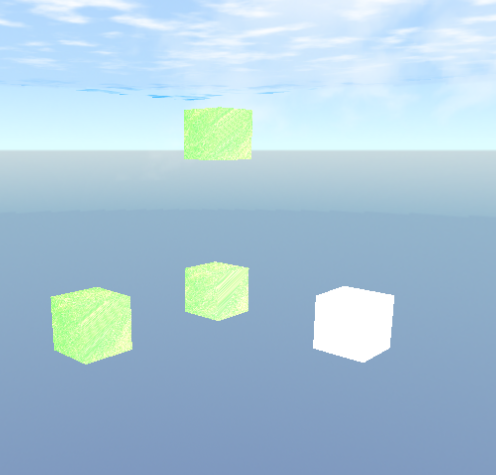
\includegraphics[scale=.4]{before_bloom}
	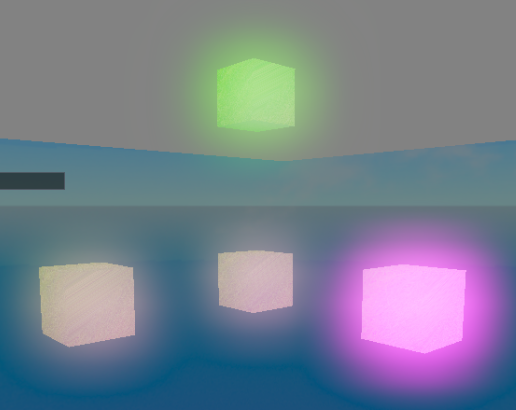
\includegraphics[scale=.47]{after_bloom}
	\caption{Exemple de cubes qui sont blanc en LDR, mais grâce au HDR et au Bloom, ont une couleur}
	\label{fig:bloom_comp_fig}
\end{figure}



\chapter{Algorithmes spécifiques}

Dans cette section nous aborderons avec plus de détails les algorithmes que nous avons dus développé et qui ont représenté des défis techniques intéressants.

\section{Affichage de l'herbe}
\label{section:grass_rendering}

Nous avons déjà abordé l'instanced rendering dans la section \ref{sec:instanced_rendering}. Néanmoins pour afficher plusieurs millions de brins d'herbe d'autres techniques sont nécessaires. On peut déjà imaginer afficher deux modèles différents, un en haute résolution (\textit{HD}) de 7 ou 8 triangles et un en basse résolution d'un seul triangle (\textit{LD}) qui sera utilisé pour les brins d'herbes loin de la caméra. On peut aussi n'afficher que les brins d'herbe visible ; on ne peut pas replacer les brins d'herbe en permanence car l'envoi de données du cpu au gpu est lent, mais on peut dire au gpu de filtrer les brins d'herbe qui ne sont pas visible pour qu'ils ne fassent pas partie de la prochaine commande d'affichage.

\paragraph{}
La méthode que nous utiliserons pour filtrer les brins d'herbe visibles est inspirée de la vidéo d'Acerola\cite{grass_rendering}. L'idée est de maintenir deux instance buffers : le complet, qui contient tous les brins d'herbe et n'est mis à jour que lorsque le joueur se déplace beaucoup pour qu'il soit toujours au milieu de la zone couverte de brins d'herbe ; et un deuxième qui contient seulement les brins d'herbe visible et est mis à jour à chaque frame. L'algorithme s'appelle le scan and compact, une version parallèle est l'algorithme \ref{alg:scan_and_compact}. Une connaissance préalable du calcul sur gpu est préférable pour comprendre cette section, expliquer le fonctionnement d'une carte graphique n'est pas du ressort de ce rapport.

\begin{algorithm}
\caption{Scan and compact}\label{alg:scan_and_compact}
\begin{algorithmic}
\State $I \gets \text{... instance buffer complet}$
\State $N \gets |I|$
\\
\State $V \gets \{0\}^N$ \Comment{Vote buffer}
\State $S \gets \{0\}^N$ \Comment{Scan buffer}
\State $B \gets \{nil\}^N$ \Comment{Compact buffer}
\State $M \gets 0$ \Comment{nombre total d'instances visibles}
\\
\ParFor{$i\gets 1, N$}
	\State $V_i \gets vote(I_i)$ \Comment{Vote, $V_i$ vaudra 1 ssi l'instance est visible}
\EndParFor
\State $S,M\gets Scan(V)$\Comment{Scan du vote buffer, cad $S_i\gets\sum_{k=1}^i V_k$}
\ParFor{$i\gets 1,N$}
	\If{$V_i=1$}
		\State $B_{S_i}\gets I_i$\Comment{Compact, les instances visibles remplissent $B$}
	\EndIf
\EndParFor
\end{algorithmic}
\end{algorithm}

L'avantage du gpu est que les calculs sont massivement parallélisables. Nous avions vu l'algorithme de scan l'année dernière en CUDA en cours. Nous n'avons pas pu récupérer l'algorithme car OpenGL permet seulement de synchroniser les threads d'un groupe et pas les groupes entre eux et nous sommes limités en nombre de threads/groupes. Concretement cela implique que l'algorithme de scan doit se diviser en trois parties parallèles. Notre implémentation est inspirée du livre GPU Gems\cite{scan_algorithm}.

\paragraph{}
En étant limité à $N=1024$ threads/groupe et $G=1024$ groupes, l'algorithme que nous proposons est limité à $G\times N=1'048'576$ brins d'herbe, et peut facilement être étendu à $G\times N^M$ en répétant $M$ fois les étapes 2 puis 3.

\begin{tabular}{|l|c|l|}
	\hline
	 & $\makecell{Threads\times\\ Groupes}$ & action\\
	\hline
	1. scan/block & $N\times  G$ & \makecell[l]{On scanne sur $V_i$ chaque block de $N$ brins\\ d'herbe, le total de chaque block est\\ stoqué dans $A_i$}\\
	\hline
	2. scan/group & $G\times 1$ & \makecell[l]{On scanne sur $A_i$ les sommes de chaque\\ block, le total est stoqué dans $M$}\\
	\hline
	3. accumulation & $N\times G$ & \makecell[l]{On ajoute à chaque valeur de chaque block\\ (les $V_i$) la somme des sommes des\\ blocks précédents (les nouveaux $A_i$)}\\
	\hline
\end{tabular}

\paragraph{}
Le code de ces algorithmes peut être trouvé dans les fichiers sous \code{res/shaders/grass/}. Le code qui les invoque se trouve dans \code{src/World/Grass.cpp}.

\paragraph{}
On peut ensuite afficher $M$ brins d'herbe. Pour arriver aux plusieurs millions promis nous exécutons cet algorithme sur \textit{deux} buffers, l'un sera affiché avec un modèle HD et le second avec un modèle LD. Il s'agit ensuite de modifier les deux instance buffers pour que les chunks proches de la caméra contiennent toujours des instances. On divise donc les deux instance buffers pour que chaque "case" contienne les instances d'un chunk. Il suffit de régénérer les cases des chunks qui changent de niveau de définition comme illustré en figure \ref{fig:grass_instance_buffers}.

\begin{figure}[H]
	\centering
	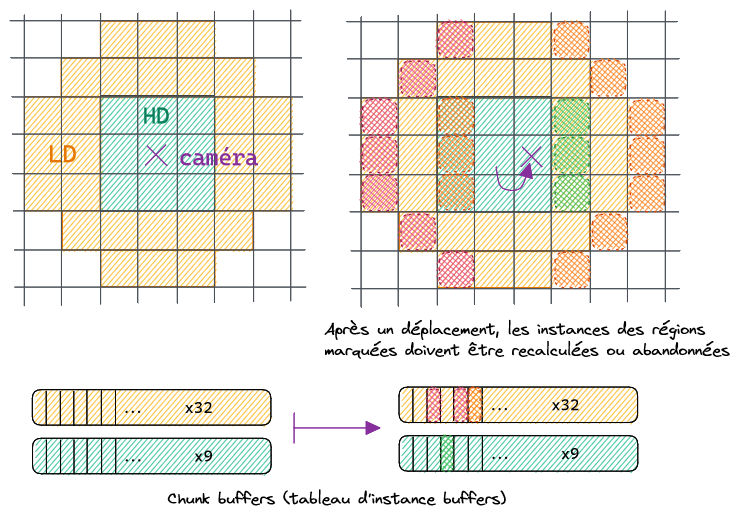
\includegraphics[scale=.49]{grass_instance_buffers}
	\caption{Les deux instance buffers de l'herbe}
	\label{fig:grass_instance_buffers}
\end{figure}

\begin{figure}[H]
	\centering
	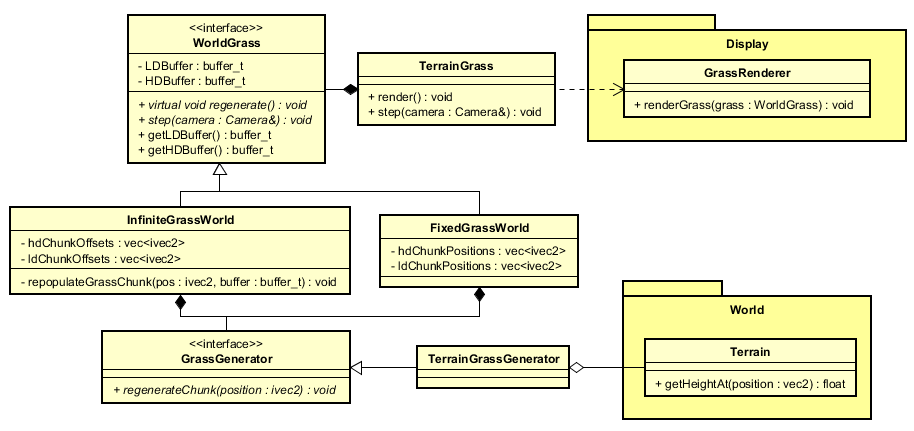
\includegraphics[scale=.49]{grass_uml}
	\caption{Diagramme de classes : composantes du système de l'herbe}
\end{figure}

Il est à noter que les chunks de l'herbe ne correspondent pas aux chunks du terrain, les deux n'ont pas les mêmes contraintes ce qui fait que généralement les chunks de l'herbe sont beaucoup plus grands. Aussi, même si nous avons implémenté la génération continue de l'herbe, nous n'avons pas fait de même pour le terrain ; cette partie du projet serait facilement réalisable mais n'entrait pas dans nos priorités. Le résultat de ces algorithmes peut être observé en figure \ref{fig:grass}.

\begin{figure}[H]
	\centering
	\caption[Capture de l'herbe]{Capture de l'herbe\\Les brins d'herbe sont très gros ici, le résultat est plus satisfaisant au loin. L'herbe est animée (le vent la déplace). Il y a environ 1M3 brins d'herbe, et 6M triangles.}
	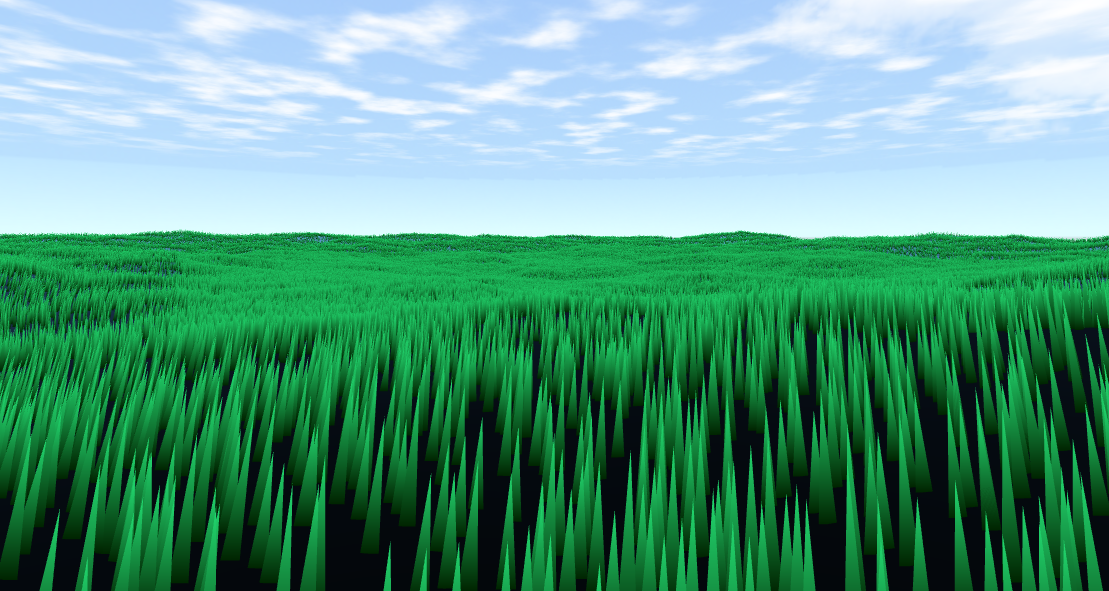
\includegraphics[scale=.35]{grass}
	\label{fig:grass}
\end{figure}

\paragraph{}
Il est assez difficile de se représenter la quantité de travail à fournir pour afficher tout cela ; si on oublie la partie "filtre" en moyenne pour 2M brins d'herbes à afficher (1M HD et 1M LD) on a $10^6\times3\times7 + 10^6\times3\times1=24\times10^6$ appels du vertex shader. Tel qu'il est écrit le vertex shader calcule deux multiplications de matrices par appel\footnote{en réalité il fait aussi plusieurs calculs trigonométriques et bien plus d'additions/multiplications, sans compter les déplacements de valeurs en mémoire...}, pour environ 20 multiplications. Au total, le gpu doit traiter (beaucoup) plus de 500M multiplications par frame, et tout cela en moins de 16ms ! Avec les optimisations que nous avons apportées dans le cas idéal (quand aucun brin d'herbe n'est dans le champ de la caméra) chaque brin d'herbe est traité en un seul calcul, mais l'algorithme possède un coût incompressible non-négligeable. On se rend bien compte de la difficulté que représente l'affichage d'autant d'objets. Ce serait complètement impossible sans gpu.

\section{Eau}

\paragraph{}
Dessiner de l'eau par ordinateur peut être une tâche très compliquée si l'on applique une approche basée sur la physique. La simulation de la mécanique des fluides et évidemment trop coûteuse, et nécessite bien souvent la génération de milliers de petites boules qui représente les molécules d'eau.
\paragraph{}
Une autre approche consiste à utiliser une grille, et effectuer les calculs sur les Vertices qui composent la grille. On utilise alors une technologie appelée Vertex Displacement, qui consiste à modifier la positions d'un vertex depuis un shader. 
C'est sur ce principe que repose les Gertsner Waves, qui simulent des comportements naturels d'un océan par exemple. Pour que cet effet soit réaliste, il faut cependant un grand nombre de Vertices, et les jeux qui utilisent ces technologies sont souvent centrées sur l'océan, la mer. On peut citer Sea of Thieves, ou encore Subnautica.

\paragraph{}
Dans notre cas, on va se contenter d'utiliser - comme bien souvent - des combines pour donner l'illusion d'eau.
\paragraph{}
Pour se faire, l'eau ne sera qu'une surface plane, composée de 4 points. Nous allons créer dynamiquement une texture et l'appliquer à cette surface.
Cette texture prendra en compte des effets de lumière, de reflexivité et réfractivité, en fonction notamment de la position de la caméra par rapport à la surface de l'eau, et celle du soleil.
Histoire que tout le monde soit au point, la réfraction, c'est ce qui se trouve sous l'eau et qui est légèrement déformé à cause de la lumière, et la réfléxion, c'est l'effet miroir.

\begin{figure}[h]
	\centering
	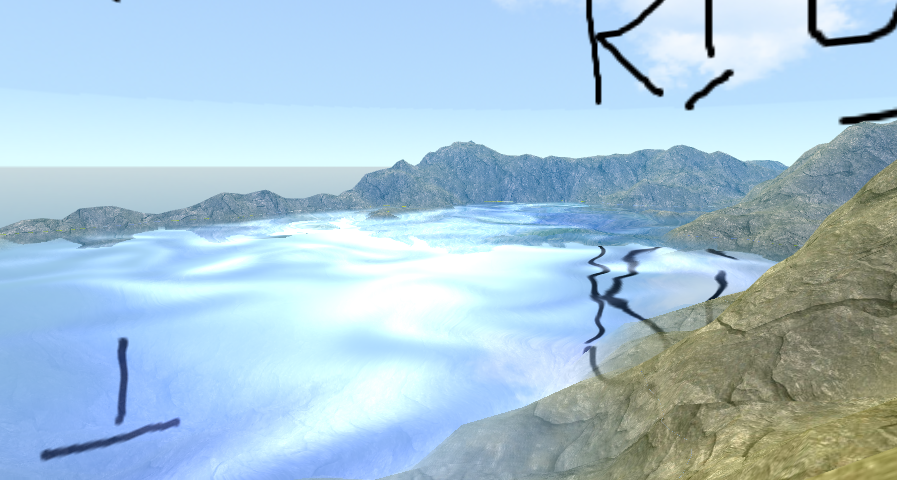
\includegraphics[scale=.6]{water}
	\caption{Résultat final de notre eau}
	\label{fig:water}
\end{figure}

Les différentes étapes pour parvenir à ce résultat sont les suivantes :


\begin{enumerate}
\item Calculer une texture de rélexion et une texture de réfraction et les combiner
\item Appliquer une texture de distortion et donner un effet de mouvement
\item Appliquer une texture de normales et calculer les jeux de lumières
\item Peaufiner le tout via l'effet Fresnel, l'utilisation d'un Z-Buffer pour lisser les bords et assombrir le fond
\end{enumerate}

\paragraph{}
La première étape est la plus couteuse de toute la procédure. L'idée est de redessiner la scène d'un autre point de vue, et d'écrire cette vue dans une texture.
Pour la réfraction, c'est le plus simple. On se contente de dessiner la scène mais uniquement ce qui se trouve en dessous du plan de l'eau.
Pour la réflexion, on place la caméra en dessous du sol et on dessine la scène mais uniquement ce qui se trouve au dessus de l'eau.
Cette étape signifie qu'on redessine 2 fois la scène en plus, ce qui peut être très lourd ! Beaucoup de jeux ne s'embètent pas à calculer la réfléction par exemple.

\begin{figure}[h]
	\centering
	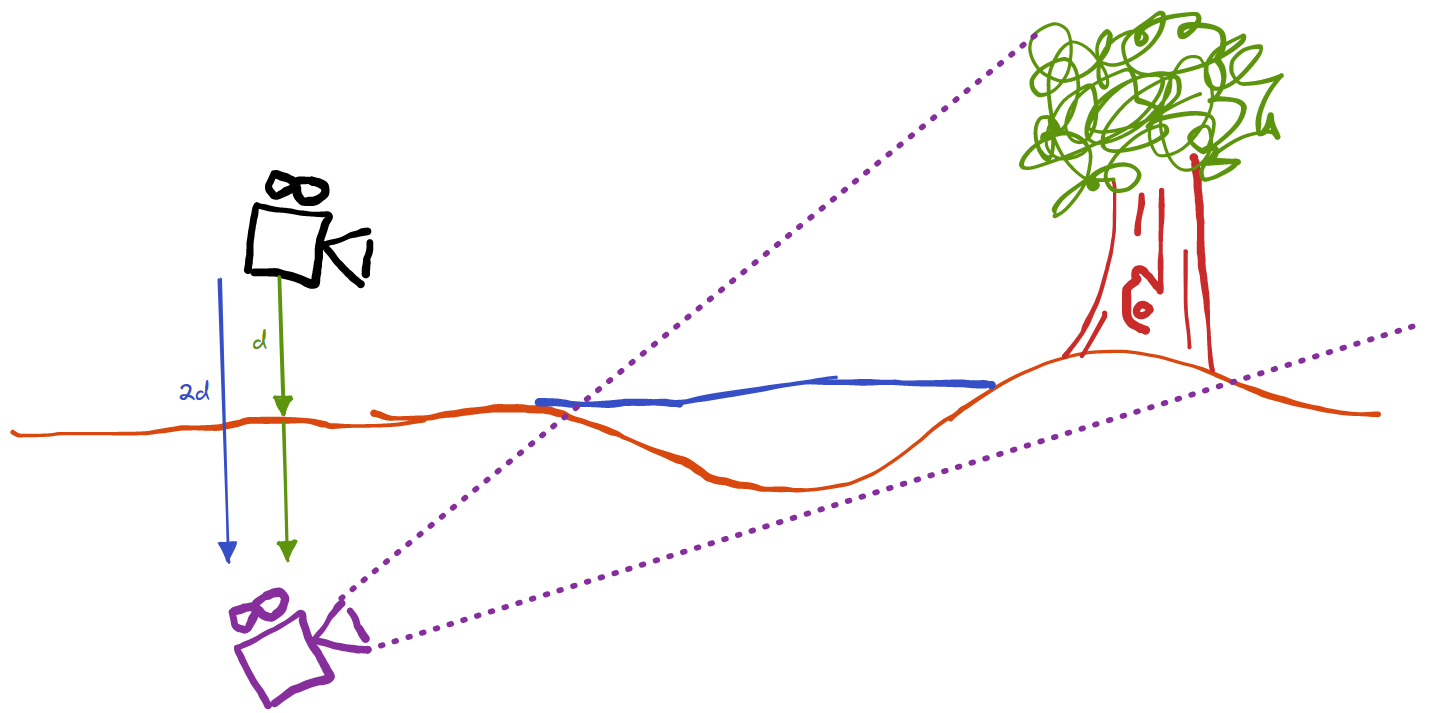
\includegraphics[scale=.3]{water_camera}
	\caption{Placement de la caméra pour les différents points de vues}
	\label{fig:water_camera}
\end{figure}

\paragraph{}
C'est bien beau tout ca... mais comment on restreint notre géométrie ? Comment peut on dire "uniquement ce qu'on trouve au dessus / dessous" ?
Heureusement pour nous, OpenGL nous fournit les Clipping Planes. Ces objets doivent être explicitement activés via \code{glEnable}.
Ensuite, on peut donner une hauteur à se plan, et OpenGL se charge, dans le Vertex Shader, de supprimer la géometrie qui se trouve sous le plan.
\begin{figure}[h]
	\centering
	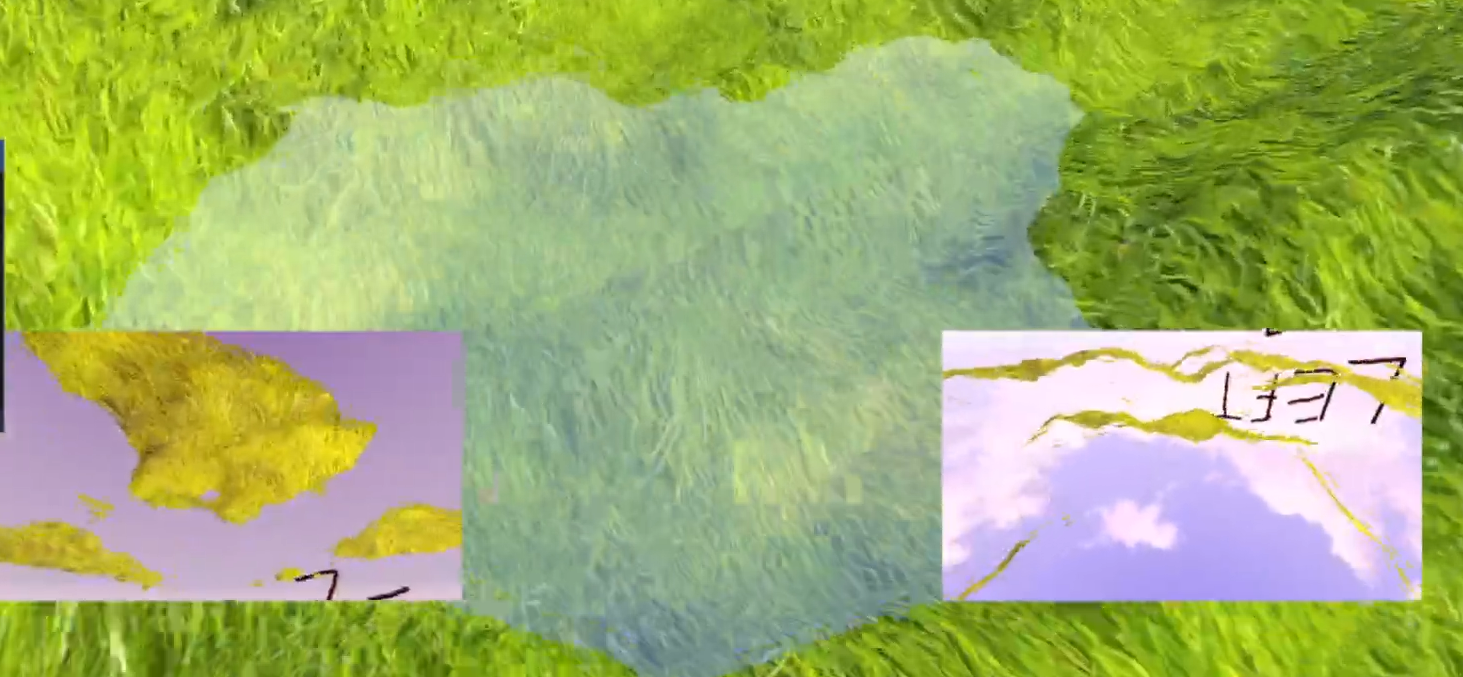
\includegraphics[scale=.3]{water_textures}
	\caption{Les deux textures obtenues. A gauche, la réflraction, à droite, la réfléxion.}
	\label{fig:water_textures}
\end{figure}

\paragraph{}
Pour la deuxième étape, on va utiliser une Distortion Map. C'est une texture qu'on va "importer" pour qu'elle soit lu dans le Fragment Shader.
Chacun des pixel de cette texture possède une certaines quantité de rouge et de vert, et cette quantité va indiquer un décalage dans la lecture de notre texture combinée dans l'étape 1.
Si l'on passe une variable de temps dans le Fragment Shader via une uniform, on peut également calculer un décalage dans la texture de distortion ! Cette astuce donne l'illusion de mouvement et de vagues.

\paragraph{}
Tant qu'à faire, on va aussi en profiter pour faire l'étape numéro 3 et calculer les lumières.
Comme toujours, la lumière se calcule avec les normales. On peut déterminer une lumière diffuse via le produit scalaire avec la normale du plan et la position du soleil, mais ce qui donne vraiment de l'impact, c'est la lumière spéculaire.
Elle se calcule en effectuant le produit scalaire du vecteur de la refléction du soleil par rapport à la normale de l'eau, et le vecteur de la caméra vers l'eau.

\paragraph{}
Afin d'obtenir une sensation de "hauteur" de l'eau, on ne peut pas se contenter de dire que la normale en chaque point est la perpendiculaire parfaite du plan.
On utilise, comme pour les mouvements, une Normal Map. Cette texture contient des informations sur la direction de la normale qui sont inscrites dans les valeurs RGB de la texture.
Cette texture est intentionnellement similaire à celle de distortion.


\begin{figure}[h]
	\centering
	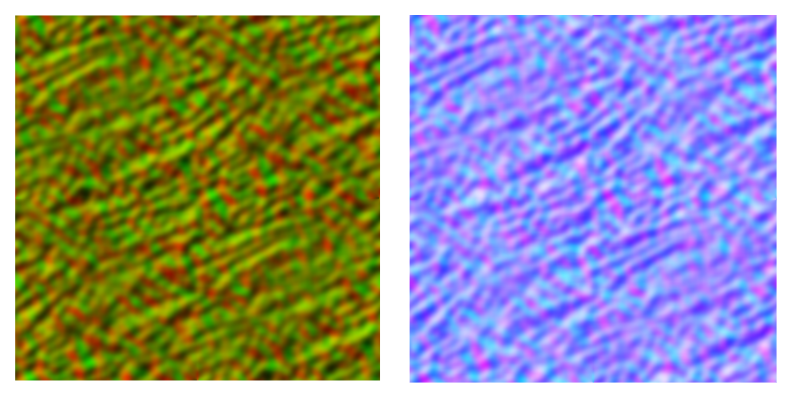
\includegraphics[scale=.4]{water_distortion_normal}
	\caption{A gauche une texture de distortion, à droite, une texture de normales}
	\label{fig:water_distortion_normal}
\end{figure}



\newtcolorbox[blend into=figures]{myfigure}[2][]{float=htb,capture=hbox,
blend before title=dash hang,title={#2},every float=\centering,#1}
\begin{myfigure}{Note : On peut utiliser les normales maps sur des textures classiques !}
	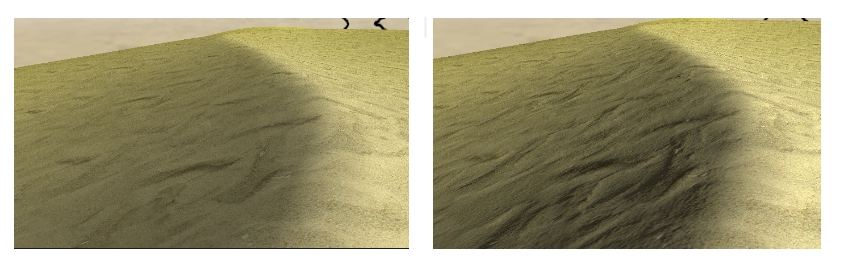
\includegraphics[scale=.6]{normals_tex}
	\label{fig:normals_tex}
\end{myfigure}


\paragraph{}
Pour la dernière étape, on pas facilement calculer l'effet Fresnel, qui dit (entre autre) que plus on est perpendiculaire à la surface de l'eau, moins cete dernière reflète (et inversement).
C'est un simple produit scalaire qui nous donne le résultat de cette loi.
\paragraph{}
Enfin, si, lors du calcul de la texture réfracteé, on en profite pour produire un depth-buffer, on peut déterminer la distance des pixels qui sont sous l'eau par rapport à la caméra. On peut donc savoir à quel point ils sont profonds dans l'eau, et ainsi appliquer
une correction de couleur pour donner un effet de profondeur !


\begin{figure}[h]
	\centering
	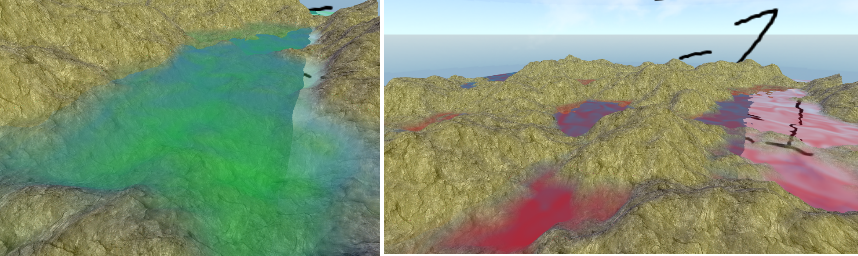
\includegraphics[scale=.5]{water_colors}
	\caption{Quelques couleurs pour l'eau...}
	\label{fig:water_colors}
\end{figure}



\chapter{Résultats}

\begin{figure}[ht]
	\centering
	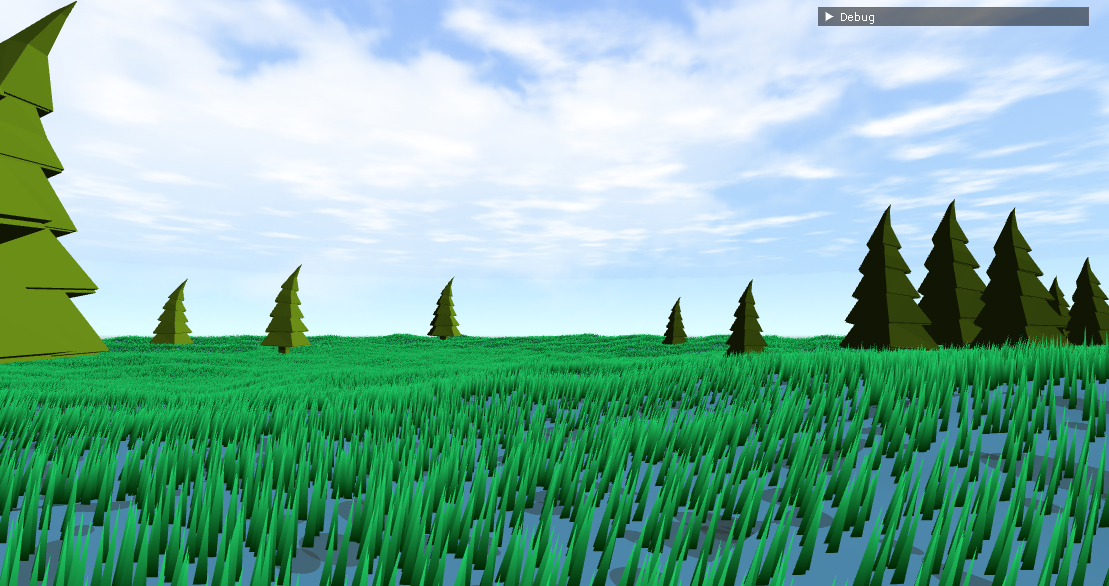
\includegraphics[height=5cm]{final_trees}
	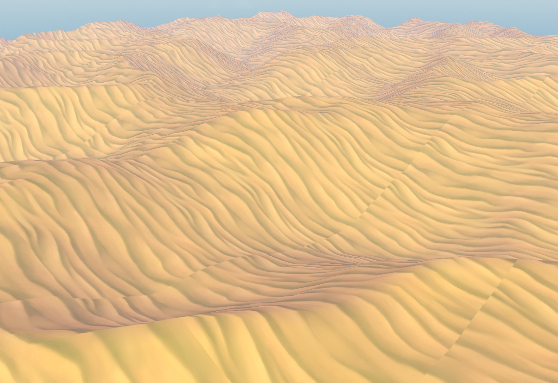
\includegraphics[height=5cm]{final_desert}
	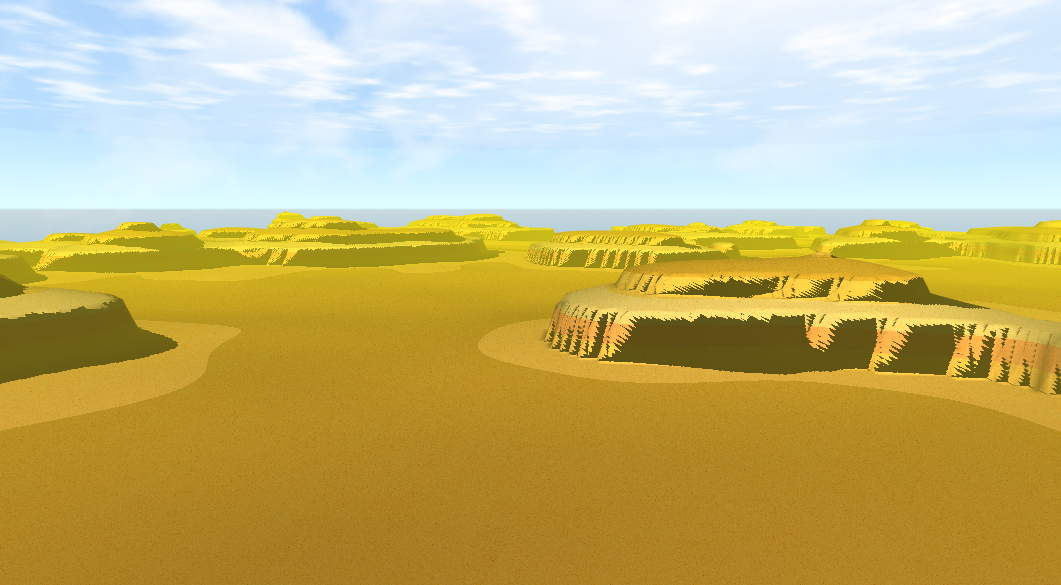
\includegraphics[height=5cm]{final_mesa}
	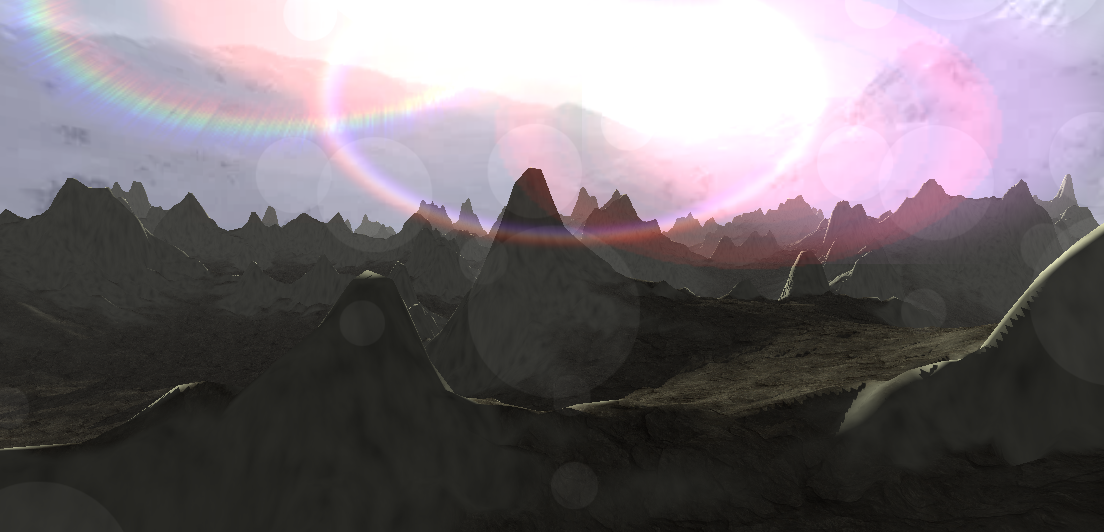
\includegraphics[height=5cm]{final_mountains}
	\caption{Captures de nos différents résultats}
	\label{fig:final}
\end{figure}

Ces visuels peuvent être obtenus en utilisant le projet dans son état final et en écrivant un peu moins de 200 lignes chacun. Le projet totalise environ $11000$ lignes de c++ et $1500$ lignes de shaders, tout cela pour arriver à un niveau d'abstraction très satisfaisant.

\chapter{Pistes d'améliorations}

Notre travail peut s'utiliser tel quel, mais le projet pourrait être poursuivi de nombreuses manières. Nous en aborderons ici quelques-unes qui nous ont paru importantes pendant le développement.

\section{Tessellation}

Le concept de \textit{tessellation} est propre à l'affichage de meshs complexes. L'idée est de répartir les vertex plus densément là où les détails sont plus importants et d'en économiser là où les détails sont moindres. Dans notre cas les vertex sont tous espacés également selon le plan $xz$ mais dès lors que les différences de niveau sont grandes on voit des artefacts apparaître. Un exemple de tessellation appliquée à un mesh de la terre peut être trouvé en figure \ref{fig:tessellation_example}.
\par
On peut aussi utiliser la tessellation de manière dynamique, en diminuant la résolution des meshs qui sont loin de la caméra. Nous l'avons fait dans une moindre mesure avec l'herbe, mais l'appliquer au terrain serait très bénéfique. Ne serait-ce que pour afficher du terrain beaucoup plus lointain.

\begin{figure}[ht]
	\centering
	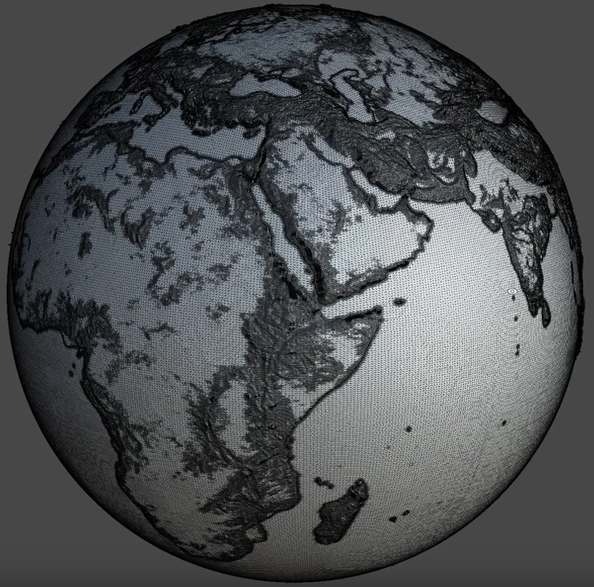
\includegraphics[scale=.4]{tessellation}
	\caption{Exemple de tessellation, les vertex sont plus denses dans les zones detailées\cite{tessellation}}
	\label{fig:tessellation_example}
\end{figure}

\section{Terrain}

Nous nous sommes focalisés sur la génération du relief du terrain, mais il reste beaucoup à faire pour créer un monde réaliste. Nous avons traité de l'eau et de l'herbe car ils représentaient des défis interessants mais rajouter des "\textit{features}" (arbres, batiments, etc...) parait essentiel. Rajouter un système de gestion de ces features performant n'est pas une mince affaire. Dans un premier temps on pourra se contenter de placer quelques modèles d'arbre dans le monde, dans un second temps on pourra les générer algorithmiquement, les animer et même concevoir un \textit{Entity Component System}\footnote{Un ECS est un système où chaque "objet" est un lien entre plusieurs composantes (physique, affichage...), chaque composante est stockée avec les autres du même type, la hiérarchie structurelle est très différente. Il est particulièrement adapté au jeu vidéo.} si les performances l'exigent.

\par
Un problème que nous avons rencontré est l'application des textures. Nous sommes passés très vite sur le sujet mais chaque vertex possède des \textit{coordonnées-uv} qui définissent la position du vertex sur une texture, notre problème vient du fait que les uvs sont calculés en fonction de la position $xz$ du vertex et ne tiennent pas compte de la hauteur. Sur des terrains très escarpés on a des artefacts importants qu'il est difficile de corriger.

\par
Une autre piste d'amélioration est la création de nuages réalistes. Nous nous sommes contenté d'utiliser astucieusement le perlin noise mais des techniques plus modernes à base de perlin noise 3D existent\footnote{SimonDev, "How Big Budget AAA Games Render Clouds", \url{https://youtu.be/Qj_tK_mdRcA}}. Avec ceci réalisé il serait facile d'ajouter de la brume dans des canyons par exemple.

\section{Physique}

Notre projet concernait seulement la génération et l'affichage, mais on peut voir facilement en quoi un moteur physique l'améliorerait. Nous avons déjà le calcul des normales et la séparation en chunks qui faciliteraient l'ajout d'un moteur physique mais le gros du travail reste à faire. Dans certaines scènes nous avons tout de même fait en sorte de simuler le déplacement du joueur sur le terrain mais notre méthode consiste seulement à replacer le joueur à une certaine distance au-dessus du mesh, il n'y a pas de réaction physique - le joueur peut gravir des montagnes au même rythme qu'il marche dans les plaines -.

\section{Géometries différentes}

Un axe assez différent d'évolution possible est la génération et l'affichage d'un monde sphérique. On pourrait imaginer créer des planètes plutôt que des mondes plats. Ajouter ce type de génération demanderait de modifier la génération des meshs et d'adapter les heightmaps pour un pavage assez spécifique (la projection du plan à la sphère est assez compliquée de manière générale) mais le reste devrait pouvoir être conservé tel quel (ombres, réflexions, génération des reliefs...).

\paragraph{}
Une autre modification qui pourrait être apportée au mesh du terrain est la modification de la grille de base, nous l'avons faite carré par soucis de simplicité mais il ne devrait pas être trop compliqué d'en faire une hexagonale. L'avantage d'une grille hexagonale est que les détails sont répartis plus homogènement, la symétrie est mieux respectée alors que les triangles des carrés font apparaître une seule des deux diagonales.

\section{Esthetiques différentes}

Nous avons choisi une esthétique qui se veut réaliste mais avec assez peu de changements on peut obtenir des visuels très différents.

\begin{figure}[ht]
	\centering
	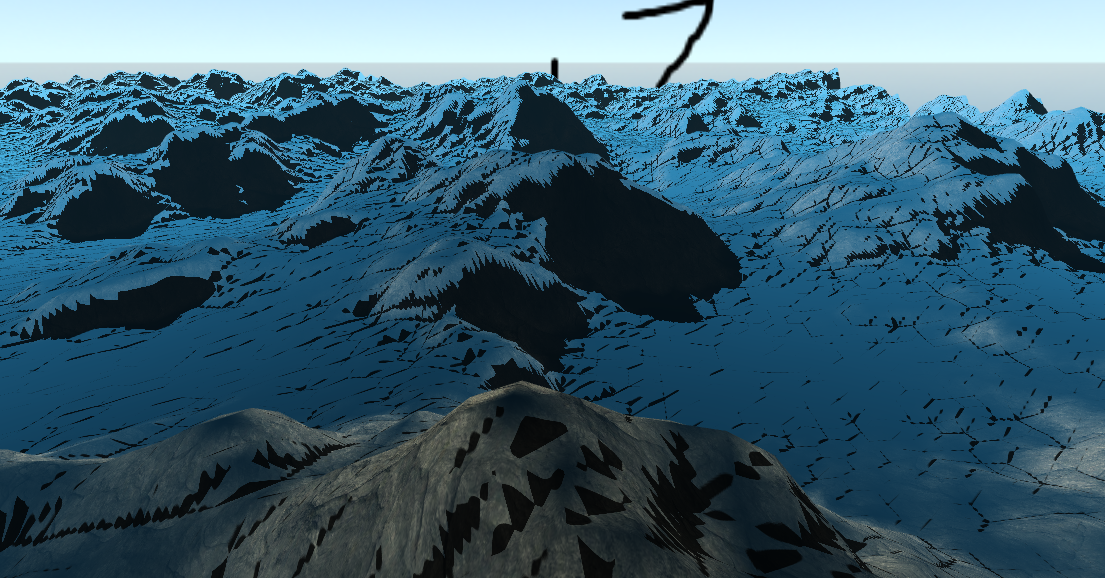
\includegraphics[scale=.205]{esthetics_1}
	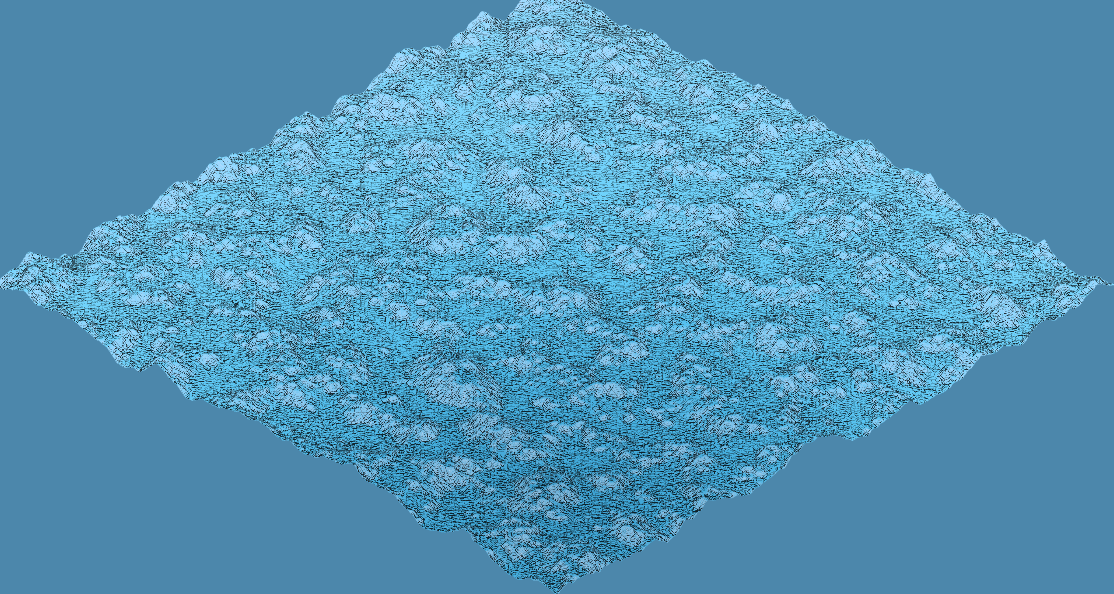
\includegraphics[scale=.2]{esthetics_2}
	\caption{Différentes variations d'esthetique}
	\label{fig:esthetics}
\end{figure}

On pourrait imaginer des visuels "low-poly" ou "toon" en diminuant le nombre de triangles et en rajoutant un shader "cel-shading\footnote{\url{https://en.wikipedia.org/wiki/Cel_shading}}".


\subsection{Volumetric Fog}

\paragraph{}
Parmi les effets de post-processing les plus impressionants et ceux qui donne le plus de réalisme, on trouve la Volumetric Fog, qui donne une excellente sensation de profondeur, d'atmosphère et apporte du réalisme aux lumières de la scène.
Cet effet est cependant très couteux... bla bla bla....

\chapter*{Conclusion}
\addcontentsline{toc}{chapter}{\numberline{}Conclusion}
\markboth{\hspace{0.5cm}Conclusion}{}

En conclusion, ce projet aura été très conséquent et instructif. Nous avons eu l'occasion de traiter bien des sujets, de la génération procédurale aux techniques d'optimisations d'affichage  très spécifiques. C'est aussi notre premier projet aussi conséquent en C++ et il nous aura fait acquérir une certaine maîtrise technique et d'architecture logicielle. Le projet est tout à fait utilisable tel quel mais en prenant un certain recul il ne reste qu'un premier jet. S'il fallait le continuer nous aurions encore bien de quoi faire.

Nous nous sommes inspiré d'un bon nombre de sources et nous avons aussi conçu par nous même des algorithmes efficaces pour résoudre des problèmes généraux. Il nous aura fallu plus de quatre mois pour tout réaliser et cela en valait tout à fait la peine.

%% TODO conclusion de la conclusion

%%%%%%%%%%%%% Bibliography %%%%%%%%%%%%%%


\begin{thebibliography}{9}
\bibitem{perlinnoise}
Perlin, Ken. "Making Noise"

\bibitem{erosion}
Hans Theobald Beyer. "Implementation of a method for hydraulic erosion"

\bibitem{grass_rendering}
Acerola, "What I Did To Optimize My Game's Grass", \url{https://youtu.be/PNvlqsXdQic}

\bibitem{scan_algorithm}
GPU Gems 3, "Chapter 39. Parallel Prefix Sum (Scan) with CUDA", \url{https://developer.nvidia.com/gpugems/gpugems3/part-vi-gpu-computing/chapter-39-parallel-prefix-sum-scan-cuda}

\bibitem{tessellation}
Sebastian Lague, "Trying to Improve My Geography Game with More Real-World Data", \url{https://youtu.be/UXD97l7ZT0w?t=989}


\bibitem{bloom}
Jorge Jimenez, "Next generation post processing in Call of Duty : Modern Warfare", \url{http://www.iryoku.com/next-generation-post-processing-in-call-of-duty-advanced-warfare}



\end{thebibliography}


%%%%%%%%%%%%% Last page %%%%%%%%%%%%%%


\resume{Le projet a pour objectif de dessiner un terrain en 3D aléatoire en utilisant du bruit. Nous avons construit un moteur 3D en OpenGL/C++, et avons également exploré et implémenté différents procédés classiques de l'industrie du jeu-vidéo pour améliorer le réalisme et les possibilités d'affichage de notre moteur. Le moteur est également pensé pour faire de l'affichage en temps réel (+60 ips).}
\motcles{infographie, génération de terrain, réalisme, lumière, ombres, GPU, OpenGL, performances, optimisations, C++, rendu, affichage, bruit}
\abstract{This project's scope is to draw and generate a 3D terrain using noise. We built a 3D Engine using C++ and OpenGL, and we explored and implemented various video-game industry techniques to enhence the realism and rendering possibilities of our engine. The engine is designed to have real-time rendering performances (+60FPS). }
\keywords{computer graphics, terrain generation, realism, lights, shadows, GPU, OpenGL, performances, optimizations, C++, rendering, noise}
\makedernierepage

\end{document}
